\chapter{Dynamic Enrichment of Bayesian Small Sample, Sequential, Multiple Assignment Randomized Trial (snSMART) Design Using Natural History Data: A Case Study from Duchenne Muscular Dystrophy}
\label{chpt:chpt2}

\section{Introduction}
\label{s:intro}
\ac{DMD} is a potentially deadly inherited genetic disease with a birth prevalence of 19.8 per 100,000 live male births \citep{crisafulli2020global}. Patients often progressively lose the ability to walk or function independently and often die at a young age from lung or heart problems. There is an unmet need for effective treatments in this patient population. Existing treatments, such as corticosteroids and exon-skipping therapies, only slow down the disease progression. Given the limited number of patients affected by \ac{DMD}, it is difficult to follow the traditional drug development paradigm, which includes separate well-controlled and well-powered dose-finding and randomized confirmatory trials. Beyond small sample sizes, variability in progression, ability to keep the blind, and ethical issues with long-term follow-up complicate the use of placebo controls in rare disease trials \citep{MUNTONI2022271}. 

Drug developers and regulators have recently shown interest in integrating external control in clinical trials to decrease the number of participants in the control arm. In the recent Rare Disease Guidance \citeyearpar{fda}, the \ac{FDA} recognizes well-designed natural history studies as a possible source of external control data in rare disease clinical trials. The \ac{CINRG} conducted the largest prospective multicenter natural history study to date in \ac{DMD}, the \ac{DNHS}. Other studies include the PRO-DMD-01 prospective natural history study (NCT01753804) and the University College London natural history study (NCT02780492), with other \ac{DMD} studies accessed through the \ac{cTAP} consortium. However, these data are rarely used in clinical trial design and analysis.

External control data is available in different forms, including patient-level data or summary-level information. Depending on the form of the data, many statistical methods, frequentist and Bayesian, have been developed to integrate external control data in clinical trials. Notable frequentist approaches include the propensity score-based approaches by \cite{rosenbaum1983central} and the test-then-pool approach by \cite{viele2014use}. Bayesian approaches include the bias model by \cite{pocock1976combination}, the power prior by \cite{ibrahim2000power}, the commensurate prior by \cite{hobbs2011hierarchical}, and meta-analytic prior by \cite{spiegelhalter2004bayesian, neuenschwander2010summarizing, schmidli2014robust} and \cite{neuenschwander2016use}. All of the Bayesian methods mentioned here discount the external information when integrating heterogeneous data sources.
 
We develop a new \ac{snSMART} design that enables formal use of external control in treatment effect estimation. Furthermore, data across two trial stages are combined using a model-based approach, which results in more precise estimates of the treatment effects. Recent years have seen substantial progress on the development of statistical models for analyzing \ac{snSMART} data: \ac{snSMART} with three active treatments when outcomes are binary \citep{wei2018bayesian, wei2020sample, chao2020dynamic} or continuous \citep{hartman2021design}, group sequential \ac{snSMART} where an active treatment arm may be removed \citep{chao2020bayesian}, and \ac{snSMART} with placebo and dose levels when outcomes are binary \citep{fang2021bayesian} or continuous \citep{fang2022comparing}. However, none of the existing \ac{snSMART} designs formally incorporate external control data, and none of the aforementioned methods enables robust integration of control data from multiple sources. Motivated by the \ac{DMD} setting, we aim to fill this gap by proposing an \ac{snSMART} that formally incorporates external control data so that the number of participants on the placebo arm can be reduced. In addition, we develop a robust, exchangeable, hierarchical model that uses all information from external controls and both stages from the \ac{snSMART} to increase the efficiency of the treatment effect estimators.

The proposed analytic method provides efficient estimates of treatment efficacy as presented in sections \ref{s:intro} and \ref{s:methods}. The simulation studies conducted to test the properties of our method are presented in section \ref{s:simulation}. Section \ref{s:results} presents the performance of different methods under various simulation scenarios. A reanalysis of the SPITFIRE trial using \ac{DNHS} data as the source of external control data is presented in section \ref{s:example} to illustrate the practical utility of the proposed methodology. Finally, we conclude with a discussion that summarizes and extends the presented \ac{snSMART} design and methods, demonstrating their power in drug discovery for other rare diseases outside of \ac{DMD}.

\section{SPITFIRE Trial: A Motivating Example of Phase IIb/III Trial in DMD}
\label{s:motivating}
This work is motivated by the current practice of \ac{DMD} drug development \citep{hoffman2019vamorolone, clemens2020safety, lake2021bayesian}. For illustration purposes, we have considered the SPITFIRE trial (NCT03039686) sponsored by \citeauthor{roche}. We use its trial setting to demonstrate the utility of the proposed approach for design and analysis to the practitioners. We have no intention to comment on or judge the clinical activity of the treatments involved or any decisions by sponsors associated with the trial or compound. The SPITFIRE trial was a randomized, 2-phase, double-blind, placebo-controlled study (See Figure \ref{fig:codatasnSMART} (a)), which assessed the efficacy, safety, and tolerability of 2 dose levels of a new therapy (RO7239361) in 6-11 years old, ambulatory boys with \ac{DMD}. In stage 1, participants were randomized to receive one of two doses of RO7239361 or placebo (1:1:1 across the three treatment arms) for 48 weeks. After completion of stage 1, subjects entered the open-label stage in which all participants received either low or high dose RO7239361 study drug for up to 192 weeks. The primary endpoint was the change from baseline in the \ac{NSAA} total score at week 48. The change from baseline at week 48 in the \ac{6MWD} test is included as a secondary outcome measure. This study aimed to detect a between group difference of 2.5 points with 80\% power. 

The SPITFIRE design is similar to an \ac{snSMART} \citep{tamura2016small}, however differs in a few ways. In the SPITFIRE trial, a) only the participants in the control group were rerandomized in stage 2, and b) only stage 1 data was used to conduct the primary analysis. This may lead to ethical and operational challenges to keep those patients in the trial. Moreover, the current approach completely ignores the second stage data in the efficacy analysis, where the second stage data contains important information about the drug. Therefore, alternative approaches that may increase patient enrollment/retention and improve treatment effect estimation are needed.

We propose an innovative Bayesian \ac{snSMART} design as an alternative to the current approach. The new approach proposes three key improvements: a) use of external control data to reduce the sample size of the placebo arm, b) provide non-responders of the first stage low dose group an opportunity to receive higher dose, and c) a Bayesian hierarchical model for primary analysis to dynamically borrow information across both trial stages. These features are extremely attractive in the rare disease setting, where sample sizes and the opportunities to perform clinical trials are limited. Further design details are provided in the next sections.

Our proposed study design is shown in Figure \ref{fig:codatasnSMART} (b), where eligible patients are randomized with a 1:2:2 or 1:3:3 chance of receiving placebo, low dose or high dose (e.g., of RO7239361), respectively, in trial stage 1. After 48 weeks, participants' \ac{NSAA} total score and other secondary outcome measurements, e.g., \ac{6MWD}, are assessed, and they are assigned or rerandomized to either the same or a different dose of treatment depending on their initial treatment and their \ac{NSAA} total score. Here, we define a participant as a treatment responder at week 48 if their baseline \ac{NSAA} total score increases, stays the same, or does not decrease by more than 3.1 \citep{muntoni2018minimal}. Specifically, participants who received placebo in stage 1 are rerandomized with equal probability in stage 2 to either the low dose or high dose treatment arm, regardless of their stage 1 response. This is beneficial to participants in the trial because everyone receives a dose of the treatment. Participants who received low dose at stage 1 are assigned to stay on low dose if they responded in stage 1 or to switch to high dose if they did not respond. Participants who first received high dose and responded are rerandomized equally between low and high dose, whereas those who did not respond to high dose are considered off trial in the second stage to discuss further treatment options with their physician. In most settings, the rerandomization of high dose responders is a viable design option because the low dose may continue to be effective and possibly more tolerable. 

\begin{figure}
\centering
\subfloat[]{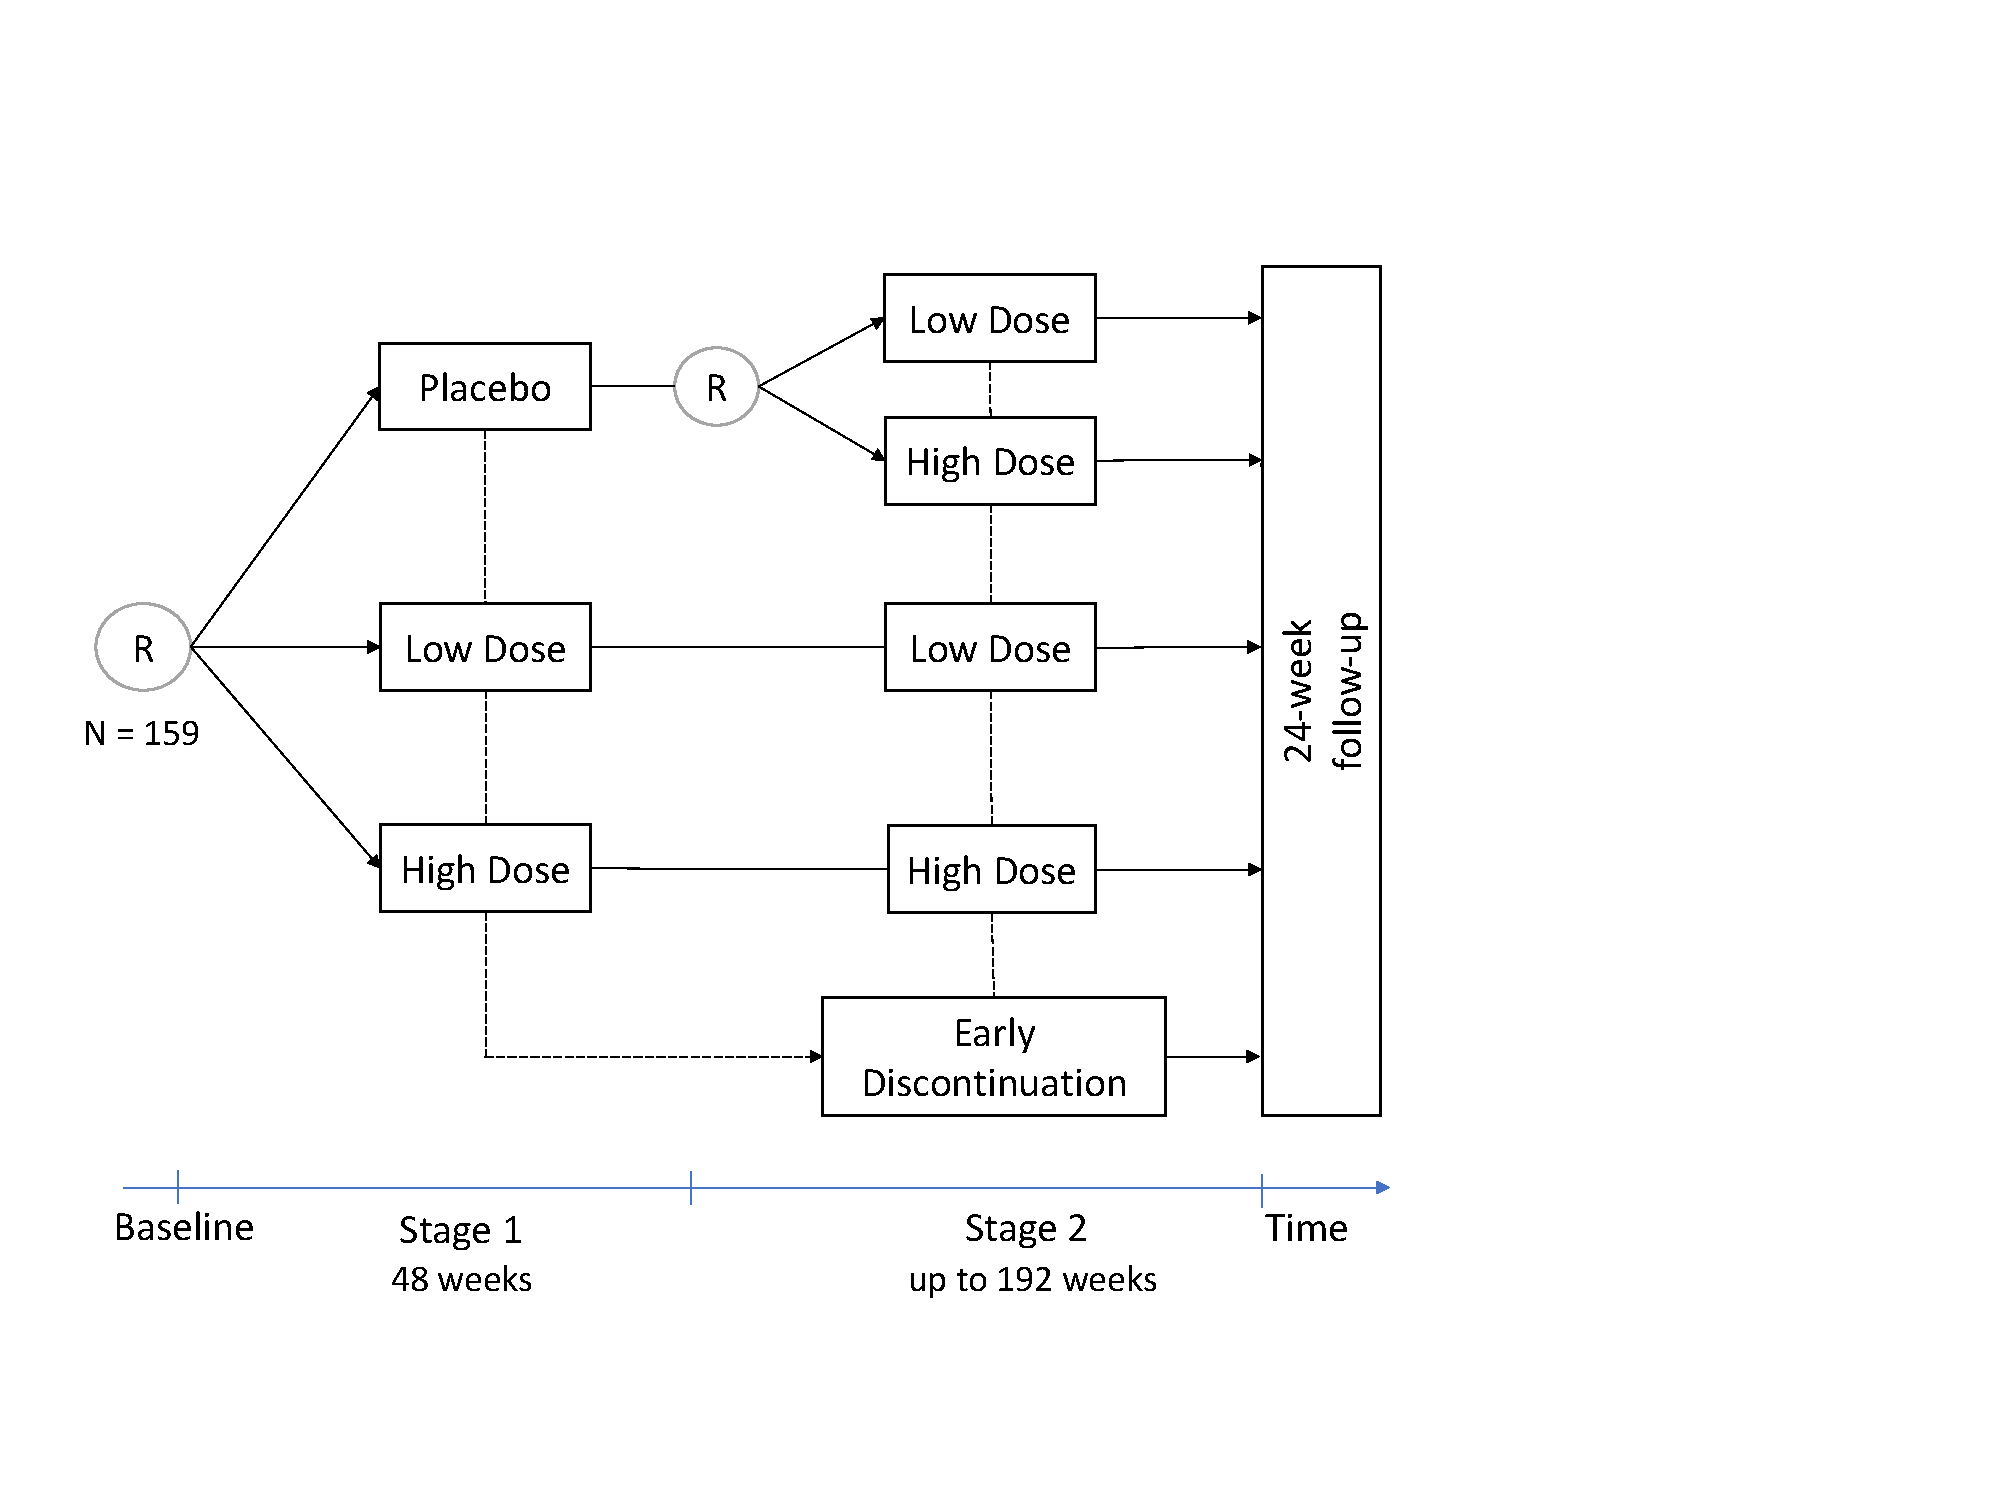
\includegraphics[width=12cm]{chapters/figures/NCT0303design.pdf}}
\\
\subfloat[]{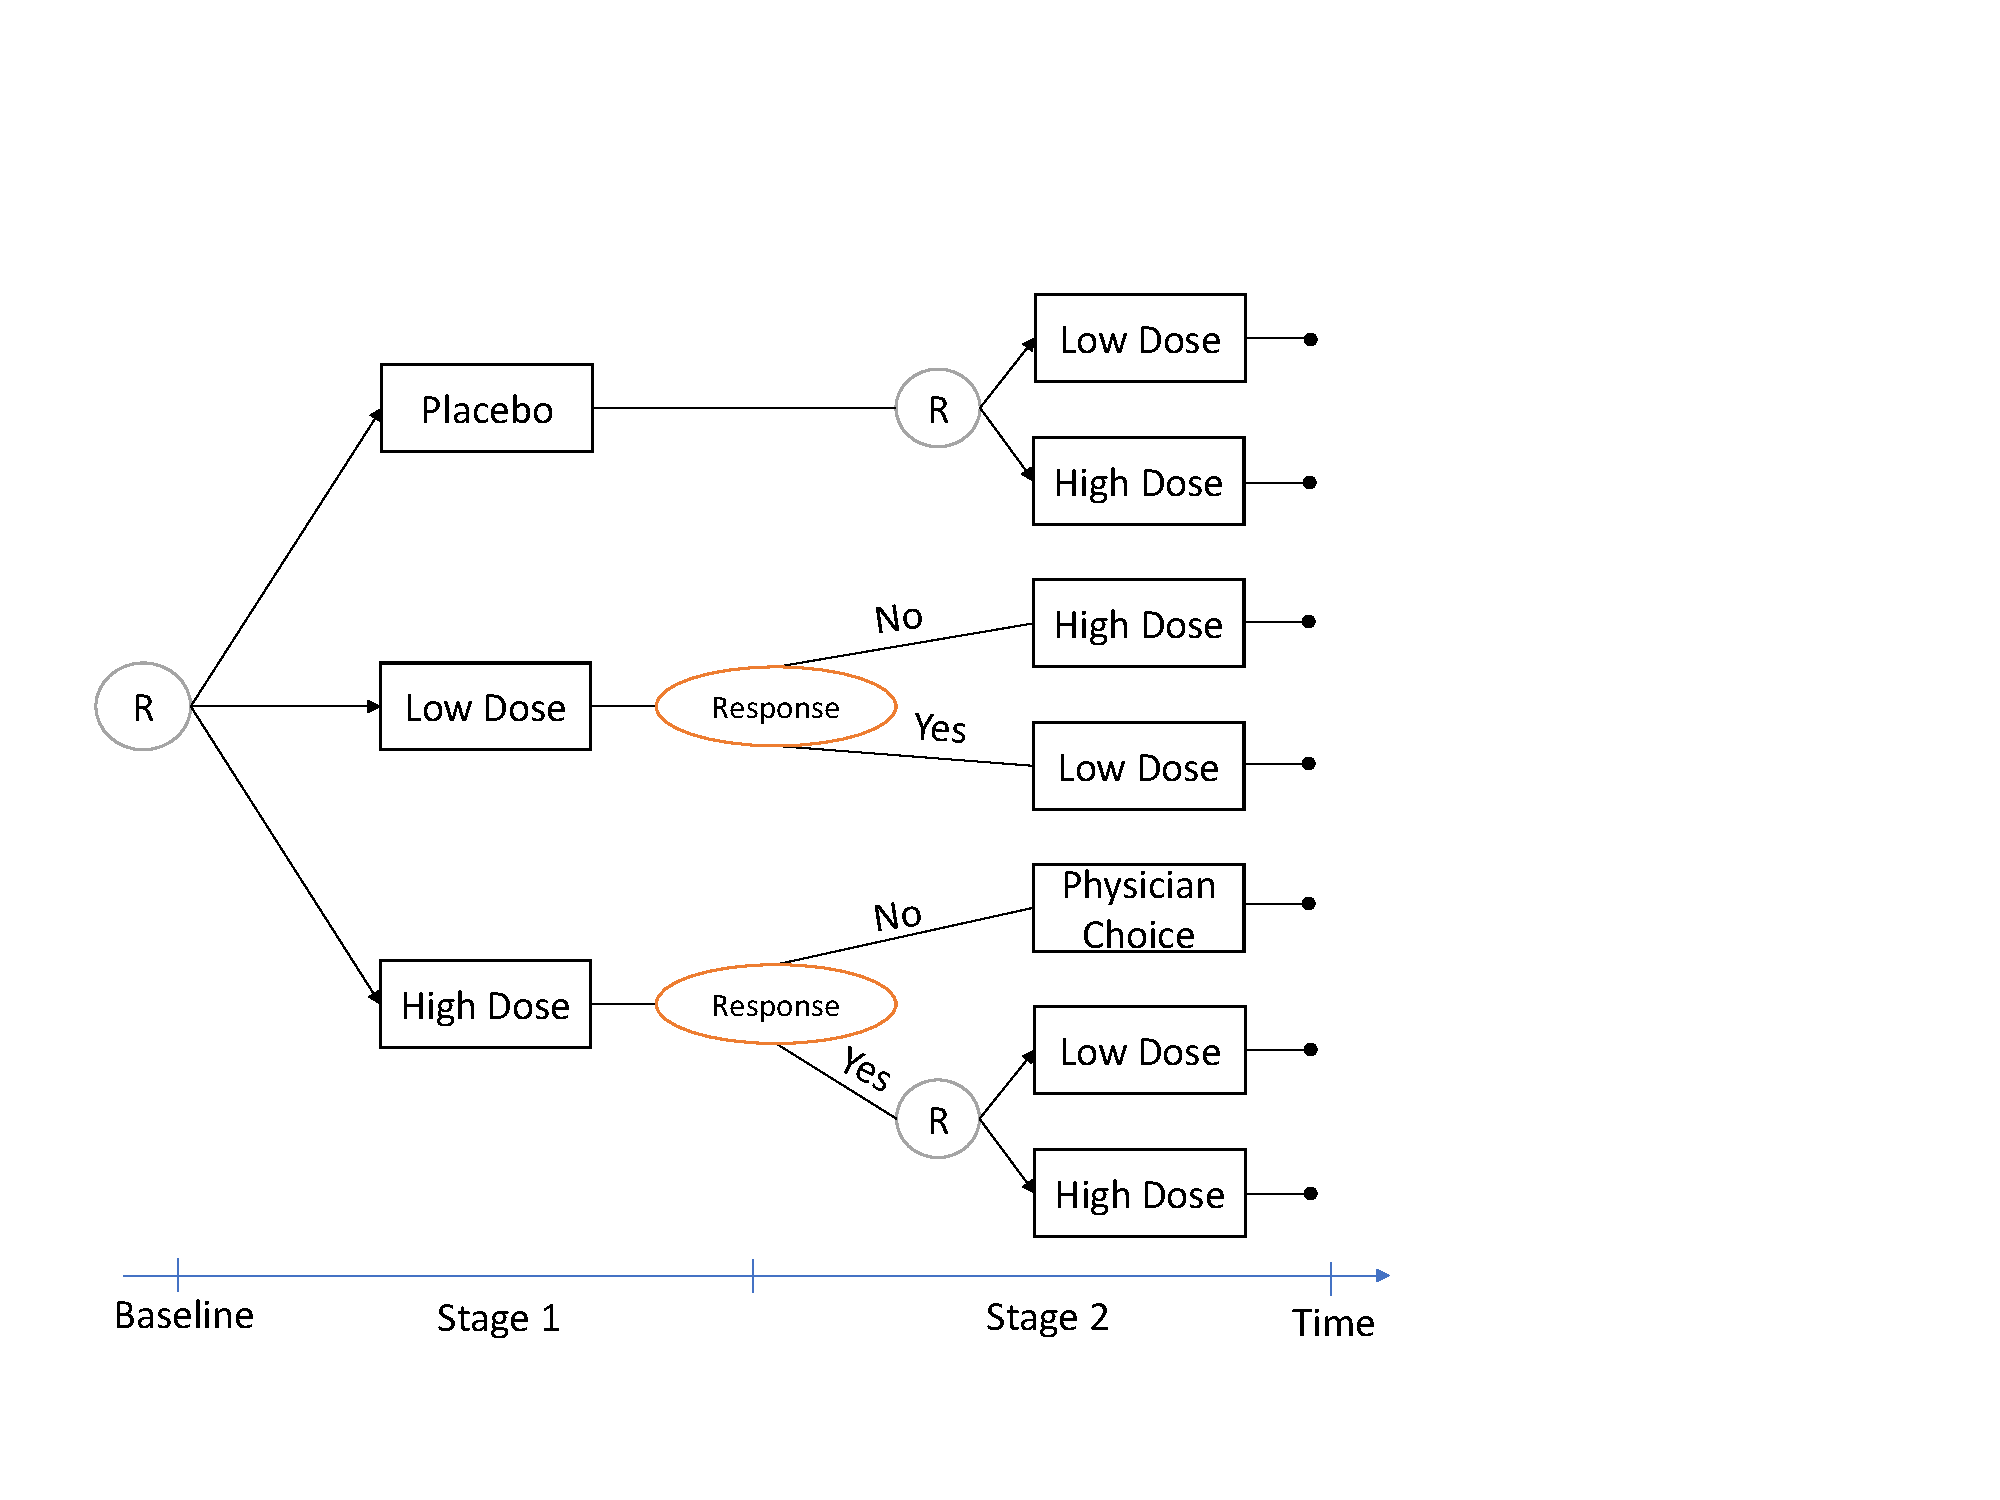
\includegraphics[width=12cm]{chapters/figures/trialdesign.pdf}}
\caption{(a) Study design of the SPITFIRE trial (NCT03039686). (R) denotes randomization. (b) Study design of the proposed \ac{snSMART} design that formally incorporates external control data. Participants are randomized (R) with 1:2:2 or 1:3:3 chances of receiving placebo, low dose or high dose, respectively, in stage 1. At the end of stage 1, participants are assigned or rerandomized to their stage 2 treatment based on their stage 1 treatment and response status. Outcomes are collected at the end of stage 1 and 2.}
\label{fig:codatasnSMART}
\end{figure}

The primary objective of the proposed \ac{snSMART} design is to estimate the stage 1 treatment effect through efficient use of data across both trial stages while formally incorporating external data. 

\section{Methods} \label{s:methods}
 
The following notation is used in this section. $Y_{jk}$ denotes the observed mean treatment effects (e.g., \ac{NSAA} total score) and $\theta_{jk}$ denotes the expected treatment effects for stage $j = 1, 2$ and treatment $k = p$ (placebo), $l$ (low dose), $h$ (high dose) respectively. For each sample of external control data $i = 1, 2, ..., n_c$, let $Y_i$ denote the observed mean placebo effect in external control data $i$, and let $\theta_i$ denote the expected mean placebo effect in external control data $i$. 

Now, we introduce the MAC-snSMART method to incorporate external control and information from both stages in \ac{snSMART} design while making inferences about stage 1. This provides a unified framework to incorporate ``all" relevant information for efficient treatment effect estimation. Here all relevant information includes external control information from any natural history studies or placebo arm data from previous trials, and trial data including placebo data in stage 1 and low/high dose information from stages 1 and 2.

\subsection{MAC-snSMART Method}
The primary goal of the proposed \ac{snSMART} design is to estimate the stage 1 treatment effects, $\theta_{1p}, \theta_{1l}$, and $\theta_{1h}$, which in our \ac{DMD} example are stage 1 mean \ac{NSAA} total score or mean \ac{6MWD}, and the difference in effects between each dose and placebo. To achieve this goal, we need to build a framework that facilitates dynamic borrowing between treatment effects, as shown in Figure \ref{fig:theta_diagram}. Challenges of this borrowing structure are apparent and require innovative solutions within the \ac{snSMART} context. Specifically, challenges include: a)  between-trial heterogeneity or conflict is inevitable given that the quality of external control data varies across studies, and b) under the proposed \ac{snSMART} design, selection bias is introduced due to non-randomized treatment assignments in stage 2 for participants who receive low dose in stage 1 and the participants who do not respond to stage 1 high dose. To tackle these two challenges, we propose a \ac{MAC}-snSMART approach with the following components.

\begin{figure}
\centering
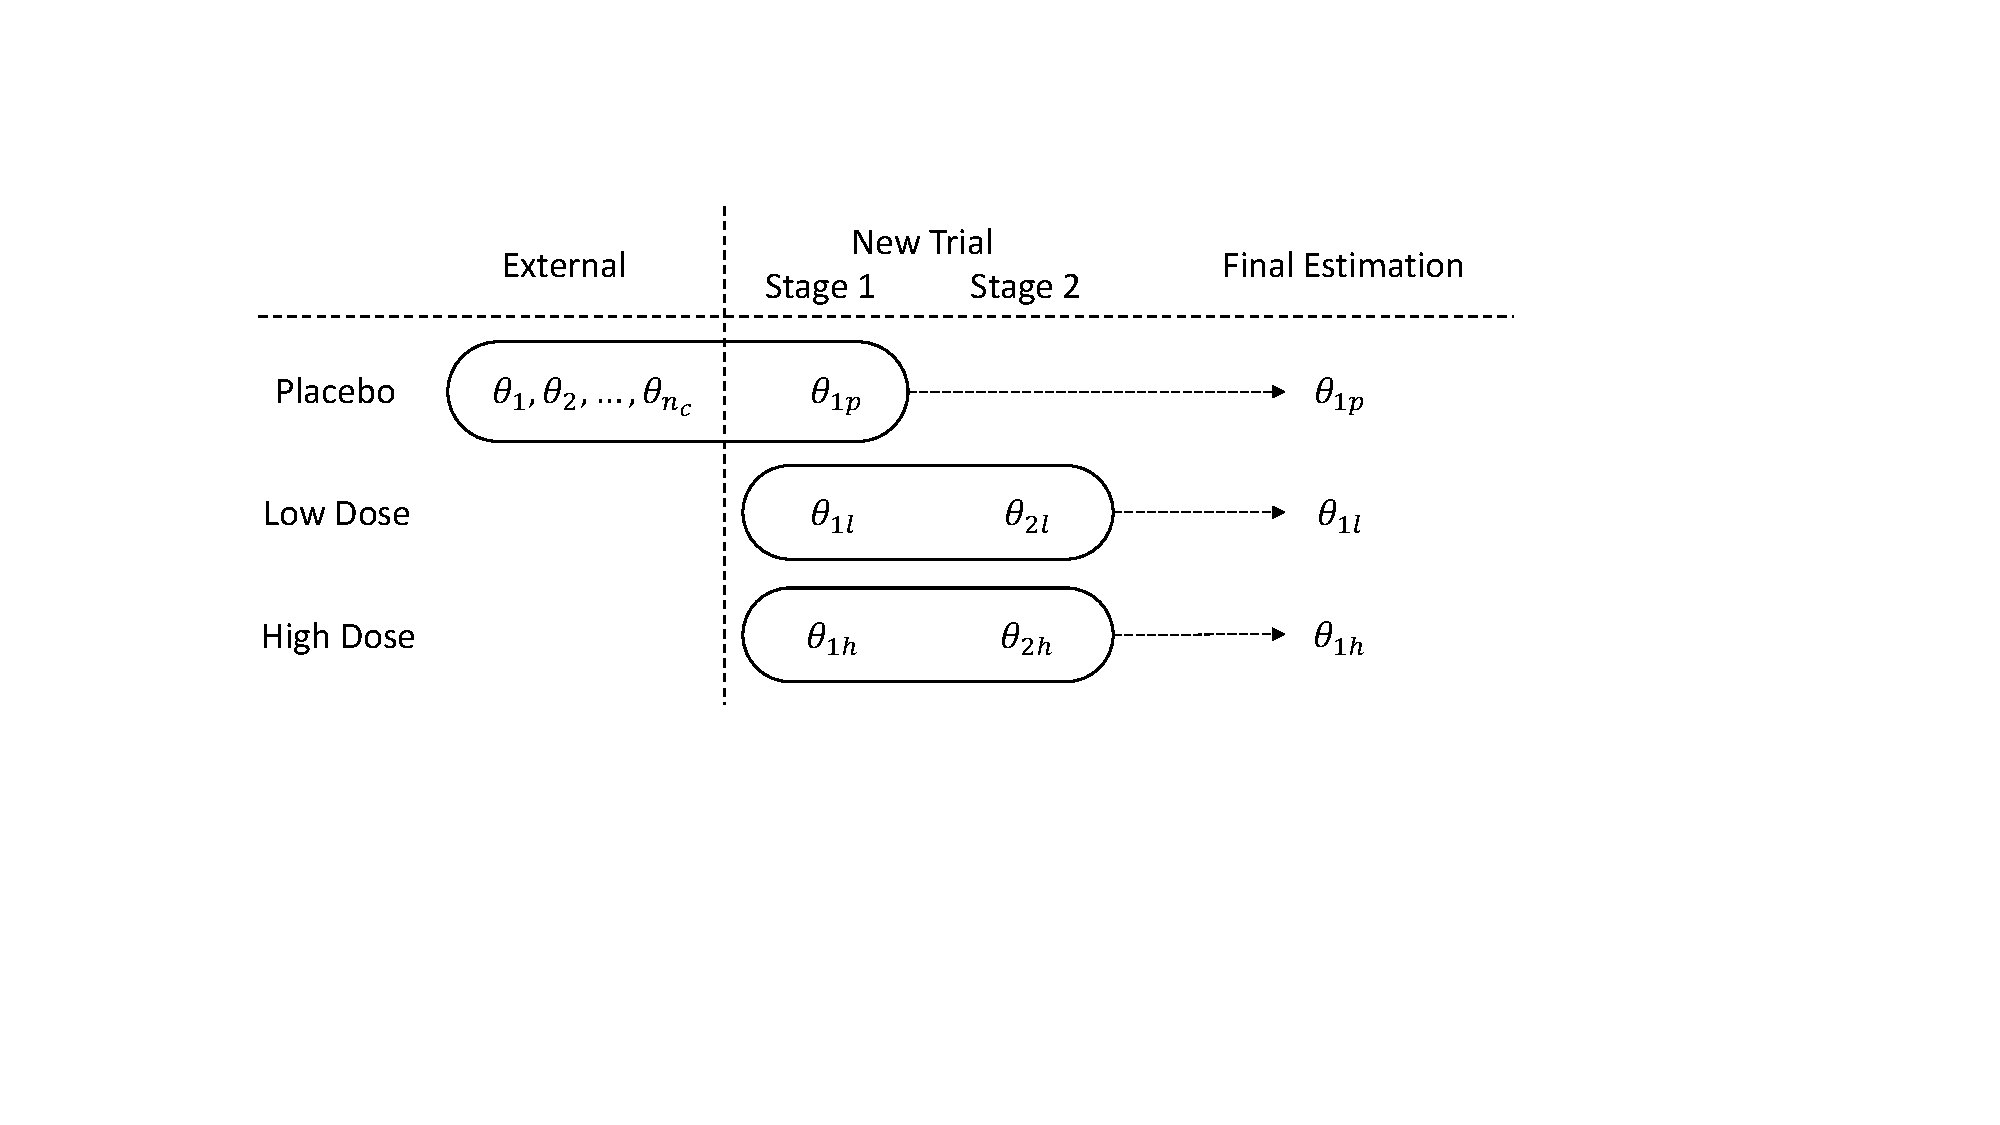
\includegraphics[width=14cm]{chapters/figures/theta_diagram.pdf}
\caption{Borrowing among treatment effects ($\theta$) in MAC-snSMART}
\label{fig:theta_diagram}
\end{figure}

\subsubsection{Combining Evidence for Placebo}
A careful selection of relevant external control data is the first critical step to control bias in the treatment effect estimate. \cite{pocock1976combination} proposed a set of criteria to assess the similarity between external control and trial control data based on the key aspects including inclusion/exclusion criteria, endpoint definition, relevance of control treatment, distribution of demographic criteria, etc. Choice of relevant external data ensures the appropriateness of the exchangeability assumption for the control parameters. Nevertheless, building a framework that acknowledges possible conflict between internal and external control is necessary to handle the effects of unmeasured confounders. 

Under the \ac{MAC}-snSMART method, $Y_i$, the observed mean placebo effect in external control data $i$, follows $Y_{i}|\theta_{i} \sim N(\theta_{i}, s_{i}^2)$, where $i = 1, 2, ...n_c$, and $s_i$ is given or derived from the $n_c$ external control data samples. Similarly, we assume $Y_{1p}|\theta_{1p} \sim N(\theta_{1p}, s_{1p}^2)$. To dynamically borrow across different studies, a parameter model is required to connect $\theta_i$ and $\theta_{1p}$. A straightforward approach to link $\theta_i$ and $\theta_{1p}$ is a hierarchical model which assumes exchangeability between internal and external control. This can be achieved by setting the same mean but a different standard deviation for each $\theta$, i.e., $\theta_{i} |\mu_p, \tau_i \sim N(\mu_p, \tau_i^2)$ and $\theta_{1p}|\mu_p,\tau_{1p} \sim N(\mu_p, \tau_{1p}^2)$. If patient-level information about important predictors is available, the model can be further extended via meta-regression. This structure accounts for external control data outliers by allowing for different between-trial standard deviations, but it could result in overly optimistic borrowing when information from different sources is non-exchangeable. 

\subsubsection{Robustification} \label{sec:robust}
To avoid overly optimistic borrowing, we include a mixture model for $\theta_i$ and $\theta_{1p}$ allowing for external control data non-exchangeability for placebo through: 
\begin{enumerate}
    \item with probability $p_{i}$, for $i = 1, 2,...,n_c$, $\theta_i|\mu_p \sim N(\mu_p, \tau_{i}^2)$; and with probability $p_{1p}$, $\theta_{1p}|\mu_p \sim N(\mu_p, \tau_{1p}^2)$
    \item with probability $1 - p_{i}$, for $i = 1, 2,...,n_c$, $\theta_i \sim N(m_i, v_i^2)$; and with probability $1 - p_{1p}$, $\theta_{1p} \sim N(m_{1p}, v_{1p}^2)$.
\end{enumerate}
A similar framework has been proposed by \cite{neuenschwander2016use}.
The prior weights $p_i$ are fixed. The values of $m_i, m_{1p}, v_i$ and $v_{1p}$ are chosen based on expert knowledge. It is essential to avoid the use of improper priors for non-exchangeability parameters ($m_{i}$, $m_{1p}$, $v_{i}$, and $v_{1p}$). Instead, weakly informative priors, such as priors worth approximately one observation \citep{kass1995reference}, should be used. 

\subsubsection{Combining Evidence for Low and High Dose Groups}

According to the proposed trial design, a participant may follow one of the seven different treatment sequences: $(1p, 2l)$, $(1p, 2h)$, $(1l, 2l)$, $(1l, 2h)$, $(1h, 2l)$, $(1h, 2h)$, and $(1h,$ \emph{No stage 2 treatment}). 
For each of the first six groups, the joint distribution of outcomes from the first and second stage, $Y_{1k}$ and $Y_{2k'}$, follows:
\begin{equation}\label{eq:joint}
\begin{bmatrix} Y_{1k} \\ Y_{2k'} \end{bmatrix} \sim MVN\left(\\ \begin{bmatrix} \theta_{1k} + b \\ \theta_{2k'}\end{bmatrix}, \begin{bmatrix} s_{1k}^2 & s_{kk'}s_{1k}s_{2k'}\\ s_{kk'}s_{1k}s_{2k'} & s_{2k'}^2\end{bmatrix}\right),
\end{equation}   
where $k = p, l, h; \ k' = l, h$. Note, $b$ is a bias correction term, which is used to adjust for the selection bias issue discussed above and further defined below. $s_{jk}$ can be estimated based on observed data in the current \ac{snSMART}. $s_{kk'}$ denotes the correlation between stage 1 treatment $k$ outcomes and stage 2 treatment $k'$ outcomes. 

Under the \ac{MAC}-snSMART approach, the conditional distribution of $\theta_{jk}$ follows that:
\begin{equation}\label{eq:theta}
   \theta_{1k},\theta_{2k} \sim N(\mu_k, \tau_k^2); \quad k = l, h \\
\end{equation}
given that we assume stage 1 and stage 2 expected outcomes for the same treatment follow the same normal distribution. Here, we explicitly define the bias correction term $b$ as:
\begin{equation}
b = I(k = l, k' = l)b_{ll} - I(k = l, k' = h)b_{lh} - I(k = h)b_{h}.
\end{equation}
Explicitly, $b_{ll}$ denotes the expected difference between the stage 1 mean treatment effect of group $(1l, 2l)$ and the overall stage 1 low dose mean treatment effect, $b_{lh}$ denotes the expected difference between the stage 1 mean treatment effect of group $(1l, 2h)$ and the overall stage 1 low dose mean treatment effect, and similarly, $b_h$ denotes the expected difference between the stage 1 mean treatment effect of high dose responders and the overall stage 1 high dose mean treatment effect. $B_{ll}, B_{lh}$ and $B_h$, the observed differences corresponding to $b_{ll}, b_{lh}$ and $b_h$, follow normal distributions $N(b_{ll}, \xi_{ll}^2)$, $N(b_{lh}, \xi_{lh}^2)$ and $N(b_h, \xi_{h}^2)$, respectively. 

\subsubsection{Prior Specification}
We suggest weakly informative normal distributions as priors for $\mu_p$ and $\mu_{k}$, weakly informative uniform distributions or normal distributions as priors for $b_{ll}, b_{lh}$ and $b_h$, and weakly informative $Unif(-1,1)$ prior distributions for $s_{kk'}$.

Half-normal priors with standard deviations roughly equal to $s_i/2$, $s_{1p}/2$ and $s_{jk}/2$ for $\tau_i$, $\tau_{1p}$ and $\tau_k$, respectively, are used to cover very small to large between-trial heterogeneity \citep{spiegelhalter2004bayesian}. According to the bias-corrected meta-analysis model proposed by \cite{verde2021bias}, roughly four participants worth of information is provided by the priors of the bias parameter. Hence, we recommend half-normal priors with standard deviation roughly equal to $s_{1l}/4, s_{1l}/4$ and $s_{1h}/4$ for $\xi_{ll}, \xi_{lh}$ and $\xi_h$, respectively. Then, the treatment effects of low dose in stage 1 and stage 2 follow the same normal distribution and are therefore exchangeable. Similarly, the high dose treatment effects in stages 1 and 2 are exchangeable.

\subsection{Posterior Distribution}
The mixture model introduced in Section \ref{sec:robust} is a mixture of normal priors. For $\theta_{1p}$, we have:
\begin{equation*}
    f(\theta_{1p}|p_{1p}, \mu_{p},\tau_{1p}, m_{1p}, v_{1p}) = p_{1p}N(\theta_{1p}|\mu_p,\tau_{1p}^2)+(1-p_{1p})N(\theta_{1p}|m_{1p},v_{1p}^2) 
\end{equation*}

Given that only summary-level treatment effect $Y_{1p}$ is used to conduct Bayesian inference, the likelihood function is the same as above. Here, we introduce the latent variable $Z_{1p}$, such that $\theta_{1p}|Z_{1p} = 1 \sim N(\mu_{p},\tau_{1p}^2)$, $\theta_{1p}|Z_{1p} = 0 \sim N(m_{1p}, v_{1p}^2)$
and $P(Z_{1p} = 1) = p_{1p}$, $P(Z_{1p} = 0) = 1-p_{1p}$.
Therefore, $Z_{1p}$ provides the label indicating the mixture components from which the observations have been generated. Now the posterior probability that $\theta_{1p}$ has been generated from $N(\mu_p, \tau_{1p}^2)$ is:
\begin{equation*}
    P(Z_{1p} = 1|\theta_{1p}, \mu_{p},\tau_{1p}, m_{1p}, v_{1p})=\frac{p_{1p}N(\mu_p, \tau_{1p}^2)}{p_{1p}N(\mu_p, \tau_{1p}^2)+(1-p_{1p})N(m_{1p}, v_{1p}^2)}.
\end{equation*}
Similarly, we could create latent variables $Z_i$ for $\theta_i$, where $i = 1, 2, ... n_c$, and use the same structure as above to obtain the posterior probability that $\theta_i$ has been generated from $N(\mu_p, \tau_i^2)$. 

Based on conjugate priors, the posterior distribution of $\theta_i$ and $\theta_{1p}$ are mixtures of normal distributions. Specifically, for $\theta_{1p}$, when equation \ref{eq:joint} is not considered, the posterior mean is:
\begin{equation*}
    p_{1p}(\eta_{1p}\hat{\mu}_p+(1-\eta_{1p})Y_{1p})+(1-p_{1p})\frac{m_{1p}(s_{1p}^2+\tau_{1p})+Y_{1p}v_{1p}^2}{s_{1p}^2+\tau_{1p}+v_{1p}^2}
\end{equation*}
where $\hat{\mu}_p = (\omega_{1p}Y_{1p} + \sum_{i}{\omega_{i}Y_{i}})/\omega_{sum}$ is the posterior mean of $\mu_p$, $\omega_i = (s_i^2+\tau_i^2)^{-1}$ and $\omega_{1p} = (s_{1p}^2+\tau_{1p})^{-1}$ are inverse variance weights, $\omega_{sum}$ is the sum of all inverse variance, and $\eta_{1p}=s_{1p}^2/(s_{1p}^2+\tau_{1p})$. 

The amount of information borrowed from external control data or second stage while estimating the treatment effects for control, low, and high dose groups can be quantified. This amount of borrowed information is sometimes expressed as effective sample size (ESS). In this manuscript, we use the expected local-information-ratio, which fulfills a basic predictive consistency requirement, as introduced by \cite{neuenschwander2020predictively}. 

\subsection{Bayesian Joint Stage Model}
The \ac{BJSM} for an \ac{snSMART} with placebo and dose levels when outcomes are continuous \citep{fang2022comparing} is an alternative way of analyzing our proposed \ac{snSMART} design. However, the \ac{BJSM} has not previously been presented to formally utilize external data. To incorporate external control data into the \ac{BJSM}, we need to calculate the effective sample size of the external control data first, then set the normal prior for the placebo treatment effect in the \ac{BJSM} to have the same effective sample size. Although the \ac{BJSM} method proposed by \cite{fang2022comparing} is designed to analyze data generated through a slightly different \ac{snSMART} design (i.e., low dose responders and non-responders are randomized and high dose non-responders continue high dose), the method itself is flexible with the number of patients on each treatment arm and the stage 2 treatment assignment rules. 
\subsection{Traditional Analytic Method}
We define a traditional analytic method for illustration purposes which mimics the method used by current, similar studies. A more traditional analytic method excludes external control data and uses only the stage 1 outcomes to estimate the stage 1 treatment effect. The SPITFIRE trial used this analytic plan to estimate the treatment effect of RO723936. Under the \ac{snSMART} design, a traditional analytic plan is structured as:
\begin{equation}\label{eq:indwo}
\begin{array}{l}
Y_{1k}|\theta_{1k} \sim N(\theta_{1k}, s_{1k}^2); \quad  k = p, l, h \\
\theta_{1k} \sim N(\mu_{1k}, \tau_{1k}^2); \quad k = l, h. \\
\end{array}
\end{equation}
Flat priors are used for $\mu_{jk}$ and $\tau_{jk}$. Other prior distributions are the same under both the robust \ac{MAC}-snSMART method and traditional method.

\section{Simulation Settings} \label{s:simulation}

We assess the sensitivity of our proposed \ac{MAC}-snSMART method to various data generating settings, possible treatment effects, exchangeability of external control data with current \ac{snSMART} data, and sample sizes. We assess two different data generation processes, one of which represents an ideal setting where data generation matches our exchangeable analytic model, and the other represents a less desirable setting where the assumption of exchangeability is violated. The first data generation process follows the assumption of the \ac{MAC}-snSMART so that $\theta_{1k}$ is set to a predetermined treatment effect and $\theta_{2k}$ is randomly generated from $N(\mu_k, \tau_k^2)$, where $\mu_k = \theta_{1k}$ and $\tau_k = 1$. Thus, the stage 1 treatment outcomes are generated based on $N(\theta_{jk}, s_{jk}^2)$ where $s_{jk} = 2$ and the stage 2 outcomes are randomly generated according to formula \ref{eq:joint}, and $s_{kk'}$ is randomly chosen within a certain range, i.e., $s_{pl} \in (-0.20, 0.20), s_{ph} \in (-0.15, 0.15), s_{ll} \in (0.70, 1), s_{lh} \in (-0.50, 0), s_{hl} \in (-0.30, 0.30)$, and $s_{hh} \in (0.70, 1)$. The second data generation process violates the assumptions of the \ac{MAC}-snSMART so that that there is no hierarchical structure (i.e., no $\mu_k$ is simulated) and $\theta_{1k}$ and $\theta_{2k}$ are not exchangeable. We set $\theta_{1k}$ to a predetermined treatment effect, and let $\theta_{2k} = \theta_{1k} + 1$. Formula \ref{eq:joint} is again used to randomly generate stage 1 and stage 2 treatment outcomes. This type of data may result from an \ac{snSMART} where a washout period between the first and second stage is inadequate. 

In addition to testing different data generation processes, we investigate the performance of our proposed models considering four treatment effect scenarios. Here, considering the \ac{DMD} context, we use a walking distance of four meters as the threshold for categorizing responders and nonresponders at the end of the stage 1. In scenario 1, we assume that the drug of interest is ineffective so that the treatment effects of placebo, low dose, and high dose are all equal to zero ($\theta_{1p} = \theta_{1l} = \theta_{1h} = 0$). In scenario 2, we assume that only the high dose is effective such that the treatment effects of placebo and low dose are zero, but high dose has a larger effect ($\theta_{1p} = \theta_{1l} = 0 < \theta_{1h} = 6$). In scenario 3, we assume that low dose has a small, but not clinically meaningful treatment effect and high dose has a clinically meaningful treatment effect ($\theta_{1p} < \theta_{1l} = 2 < \theta_{1h} = 6$). In scenario 4, we assume that low dose has a clinically meaningful effect, as does high dose ($\theta_{1p} = 0 < \theta_{1l} = 4 < \theta_{1h} = 8$). In the last scenario, to assess the sensitivity of our model to the alignment of external control and current data, we allow for $\theta_i \ne \theta_p$ for some $i$. 

Under each data generating process, 10,000 realizations per scenario were simulated. Each realization includes five sets of summary-level (mean and standard deviation) external control data (i.e., natural history of disease) and one current \ac{snSMART} dataset. Estimations from two \ac{MAC}-snSMART methods, i.e., \ac{MAC}-snSMART and robust \ac{MAC}-snSMART, and the traditional analytic method are compared. We calculate the coverage rate, \ac{rMSE}, bias, and width of the 95\% \ac{CI} of each estimator. The results section of this paper focuses on simulation results with a total sample size of 50, where 10 subjects are randomized to placebo, 20 subjects are randomized to low dose, and 20 subjects are randomized to high dose in stage 1, but results for total sample sizes of 25 are also provided in the figures.

The 95\% \ac{CI} are the narrowest intervals that include 95\% of the posterior distribution of $\theta_{jk}$, $j=1,2$, $k=p,l,h$. From scenario 1, where $\theta_{1p} = \theta_{1l} = \theta_{1h} = 0$, we define the type I error by calculating the probability that the credible intervals of $\hat{\theta}_{1l} - \hat{\theta}_{1p}$ and $\hat{\theta}_{1h} - \hat{\theta}_{1p}$ do not include 0. Similarly, from scenarios 3, 4 and 5, where the treatment effects of low and high dose are different from the treatment effect of placebo, we define power by calculating the probability that the credible intervals of $\hat{\theta}_{1l} - \hat{\theta}_{1p}$ and $\hat{\theta}_{1h} - \hat{\theta}_{1p}$ do not include 0. Model parameters are estimated via the R function jags in R package rjags \citep{rjags}.

\section{Results} \label{s:results}

For the data generation process where assumptions of exchangeability are upheld (data generating process 1), the \ac{rMSE}, bias, coverage rate, and \ac{CI} width for estimators of the expected treatment effects are shown in Figures \ref{fig:rMSE},  \ref{fig:CR}, and \ref{fig:Width}, respectively. The estimators from the \ac{MAC}-snSMART methods have smaller rMSEs than the traditional method. \ac{MAC}-snSMART methods provide similar coverage compared with the traditional method while having smaller 95\% \ac{CI} width. Even though \ac{MAC}-snSMART methods have slightly higher biases, the biases of both approaches are negligible. 
\begin{table} 
\begin{center}
\caption{\label{tab:TypeI} Simulated type I error}
\begin{tabular}{ccccccc}
\hline
\centering \multirow{2}{*}{Sample Size} & \multicolumn{2}{c}{Traditional} & \multicolumn{2}{c}{MS} & \multicolumn{2}{c}{RMS}\\
\centering  & Low & High & Low & High & Low & High \\
\hline
\textit{data generating process 1} &&&&&& \\
\raggedleft $n_{1p} = 10, n_{1l} = 20, n_{1h} = 20$ & 0.0599 & 0.0611  & 0.0452 & 0.0256 & 0.0468 & 0.0304 \\
\raggedleft $n_{1p} = 5, n_{1l} = 10, n_{1h} = 10$ & 0.0793 & 0.0745 & 0.0634 & 0.0324 & 0.0700 & 0.0374 \\
\textit{data generating process 2} &&&&&& \\
\raggedleft $n_{1p} = 10, n_{1l} = 20, n_{1h} = 20$ & 0.0664 & 0.0650 & 0.0714 & 0.0667 & 0.0730 & 0.0712 \\
\raggedleft $n_{1p} = 5, n_{1l} = 10, n_{1h} = 10$ & 0.0741 & 0.0749 & 0.0747 & 0.0569 & 0.0787 & 0.0606\\
\hline
\end{tabular}
\end{center}
\begin{tablenotes}
      \small
      \item The type I error of all presented methods is defined as the probability that the credible intervals of $\hat{\theta}_{1l} - \hat{\theta}_{1p}$ and $\hat{\theta}_{1h} - \hat{\theta}_{1p}$ do not include 0 when there are no treatment effect differences between low dose and placebo and high dose and placebo. Data generating process 1 generates datasets under the assumption that the expected treatment effect of the same dose level follows the same normal distribution across stages, and data generating process 2 generates datasets without a hierarchical structure or exchangeability between stages. $n_{1p}$, $n_{1l}$ and $n_{1h}$ denote the number of participants randomized to placebo, low dose and high dose, respectively, in stage 1. Two hierarchical models: MAC-snSMART (MS) and robust MAC-snSMART (RMS) are compared against the traditional method. 
\end{tablenotes}
\end{table}

A comparison of all metrics between the traditional method and the \ac{MAC}-snSMART methods clearly shows that estimation of the placebo effect is improved from including external control data, even when external control data is not entirely aligned with the placebo data in the current \ac{snSMART} ($\theta_{i} \ne \theta_p$ for some $i$). The robust \ac{MAC}-snSMART and the \ac{MAC}-snSMART methods provide similar estimates for low and high dose, but when external control data is not aligned with the current trial data, the placebo effect estimate is less biased under the robust \ac{MAC}-snSMART method.  

Given that stage 1 treatment outcomes are simulated with the same $n$ and the same standard deviation across scenarios with no previous treatment impact, the estimators provided by the traditional method have more stable performance across scenarios. This is in contrast to the fluctuation of metrics of the estimators provided by \ac{MAC}-snSMART methods due to the variations in $n$ and standard deviations of the stage 2 outcomes simulated under different treatment effect scenarios. 

The right column of Figures \ref{fig:rMSE}, \ref{fig:Bias}, \ref{fig:CR}, and \ref{fig:Width} present the \ac{rMSE}, bias, coverage rate, and \ac{CI} width for estimators of the treatment effects when data are generated without a hierarchical structure or exchangeability (data generating process 2). Given that the \ac{MAC}-snSMART methods borrow information across both stages, this data generation process where there is a shift in mean in stage 2 treatment effects, leads to larger positive biases and subsequently lower coverage rates and higher \ac{rMSE} values compared to the traditional method. The decrease in coverage rate can be mitigated by setting a larger standard deviation for the half-normal prior of $\tau_k$. The estimates produced by the traditional method are not affected by the mean shift in stage 2, given that only stage 1 data is used to estimate stage 1 treatment effects. Under this data generation setting, the traditional method provides the best treatment effect estimators among the presented methods. 

\begin{figure}
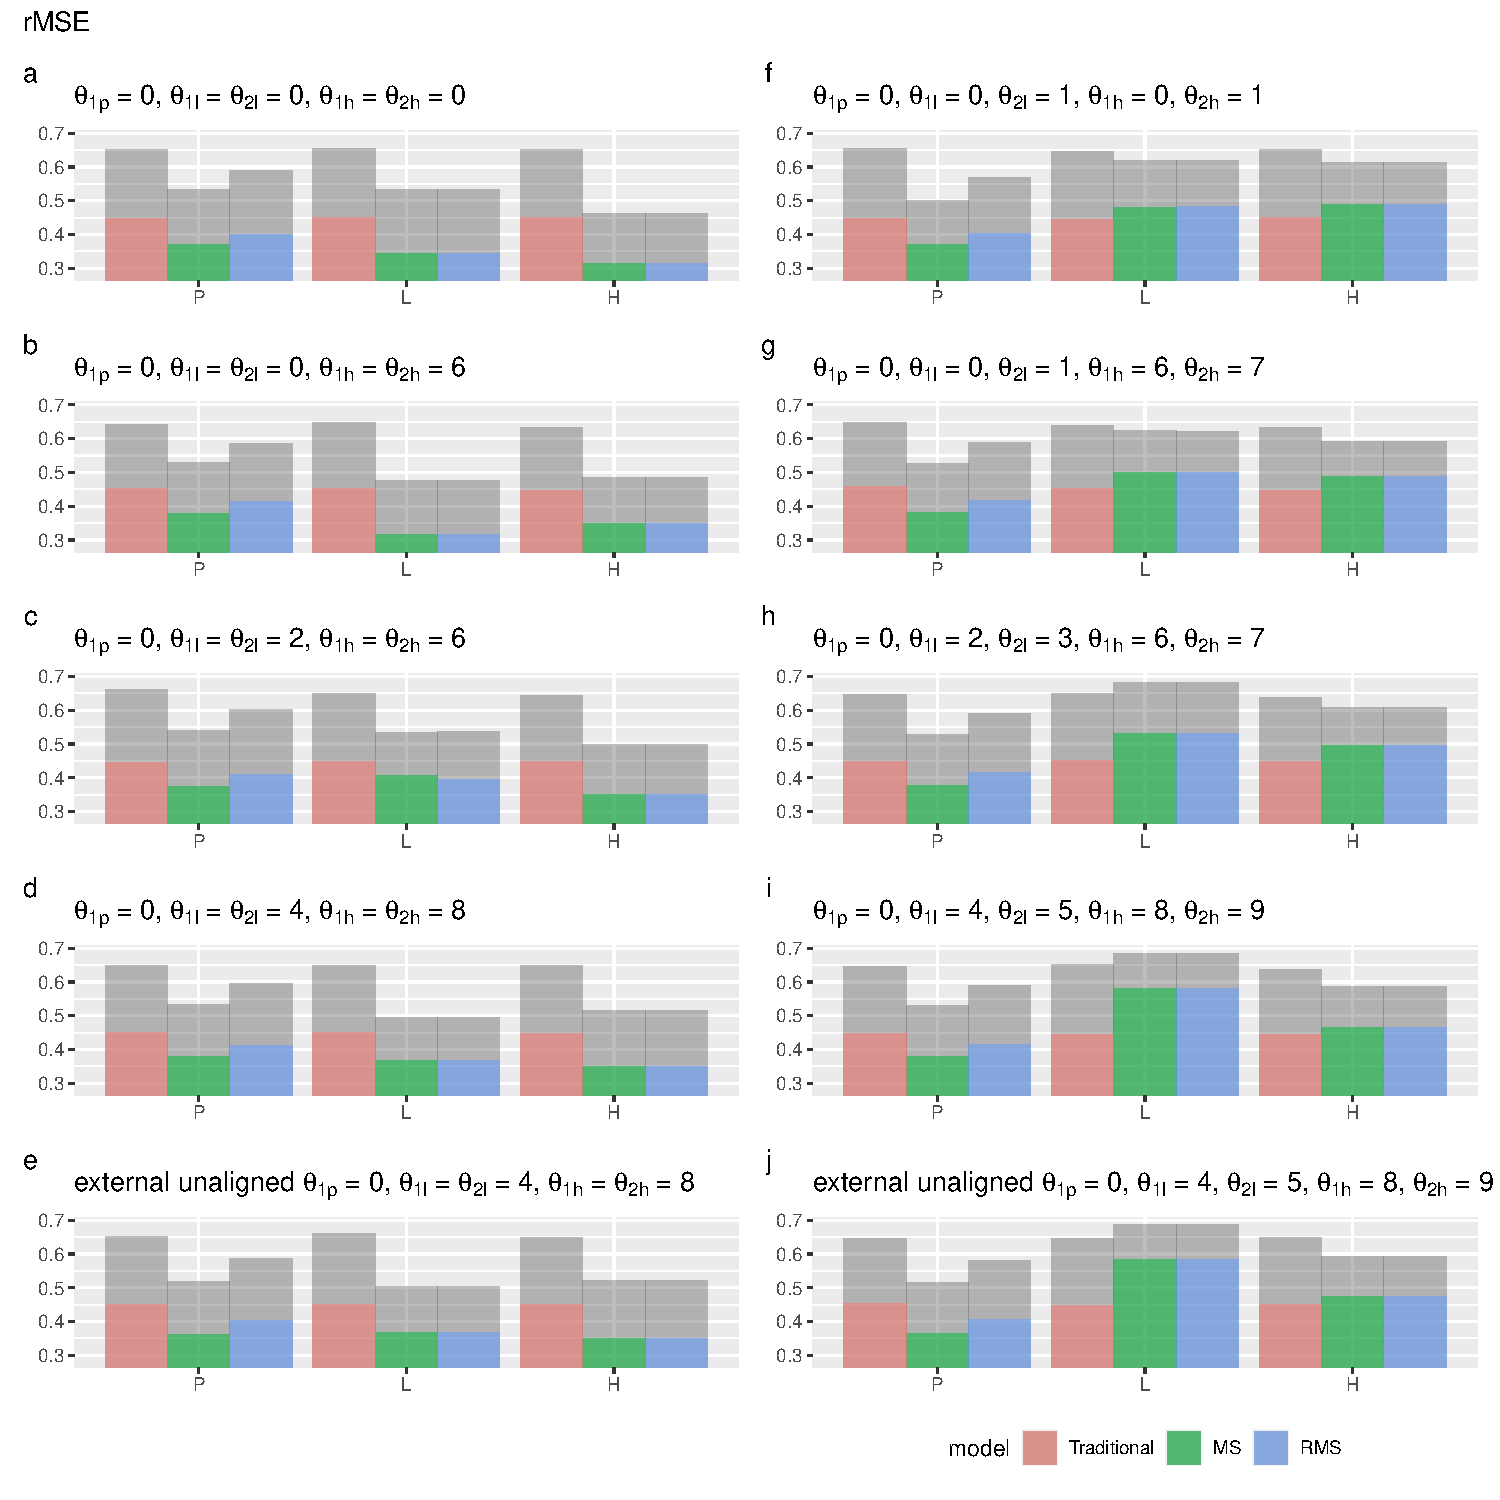
\includegraphics[width=16cm]{chapters/figures/rMSE.pdf}
\caption{Simulated root-mean-square error (rMSE) for the estimators of $\theta_{1k}$}
\subcaption*{$\theta_{jk}$ is the stage $j$ treatment effect of treatment $k$, where $j = 1,2, k = P, L, H$, P = placebo, L = low dose, and H = high dose. Two hierarchical models: MAC-snSMART (MS) and robust MAC-snSMART (RMS) methods are compared against the traditional method. The results of total sample size 50 are shown as the colored bars, while the results of total sample size 25 are shown as the overlaying grey bars. The simulation settings are described on the top of each graph, where $\theta_{jk}$ denotes the true value of the expected treatment effects of treatment $k$ in stage $j$, $j = 1, 2$, $k = P, L, H$, and \emph{external unaligned} means the placebo treatment effects in external control data are inconsistent with the placebo treatment effect in the current trial. This figure appears in color in the electronic version of this article, and color refers to that version.}
\label{fig:rMSE}
\end{figure}

\begin{figure}[H]
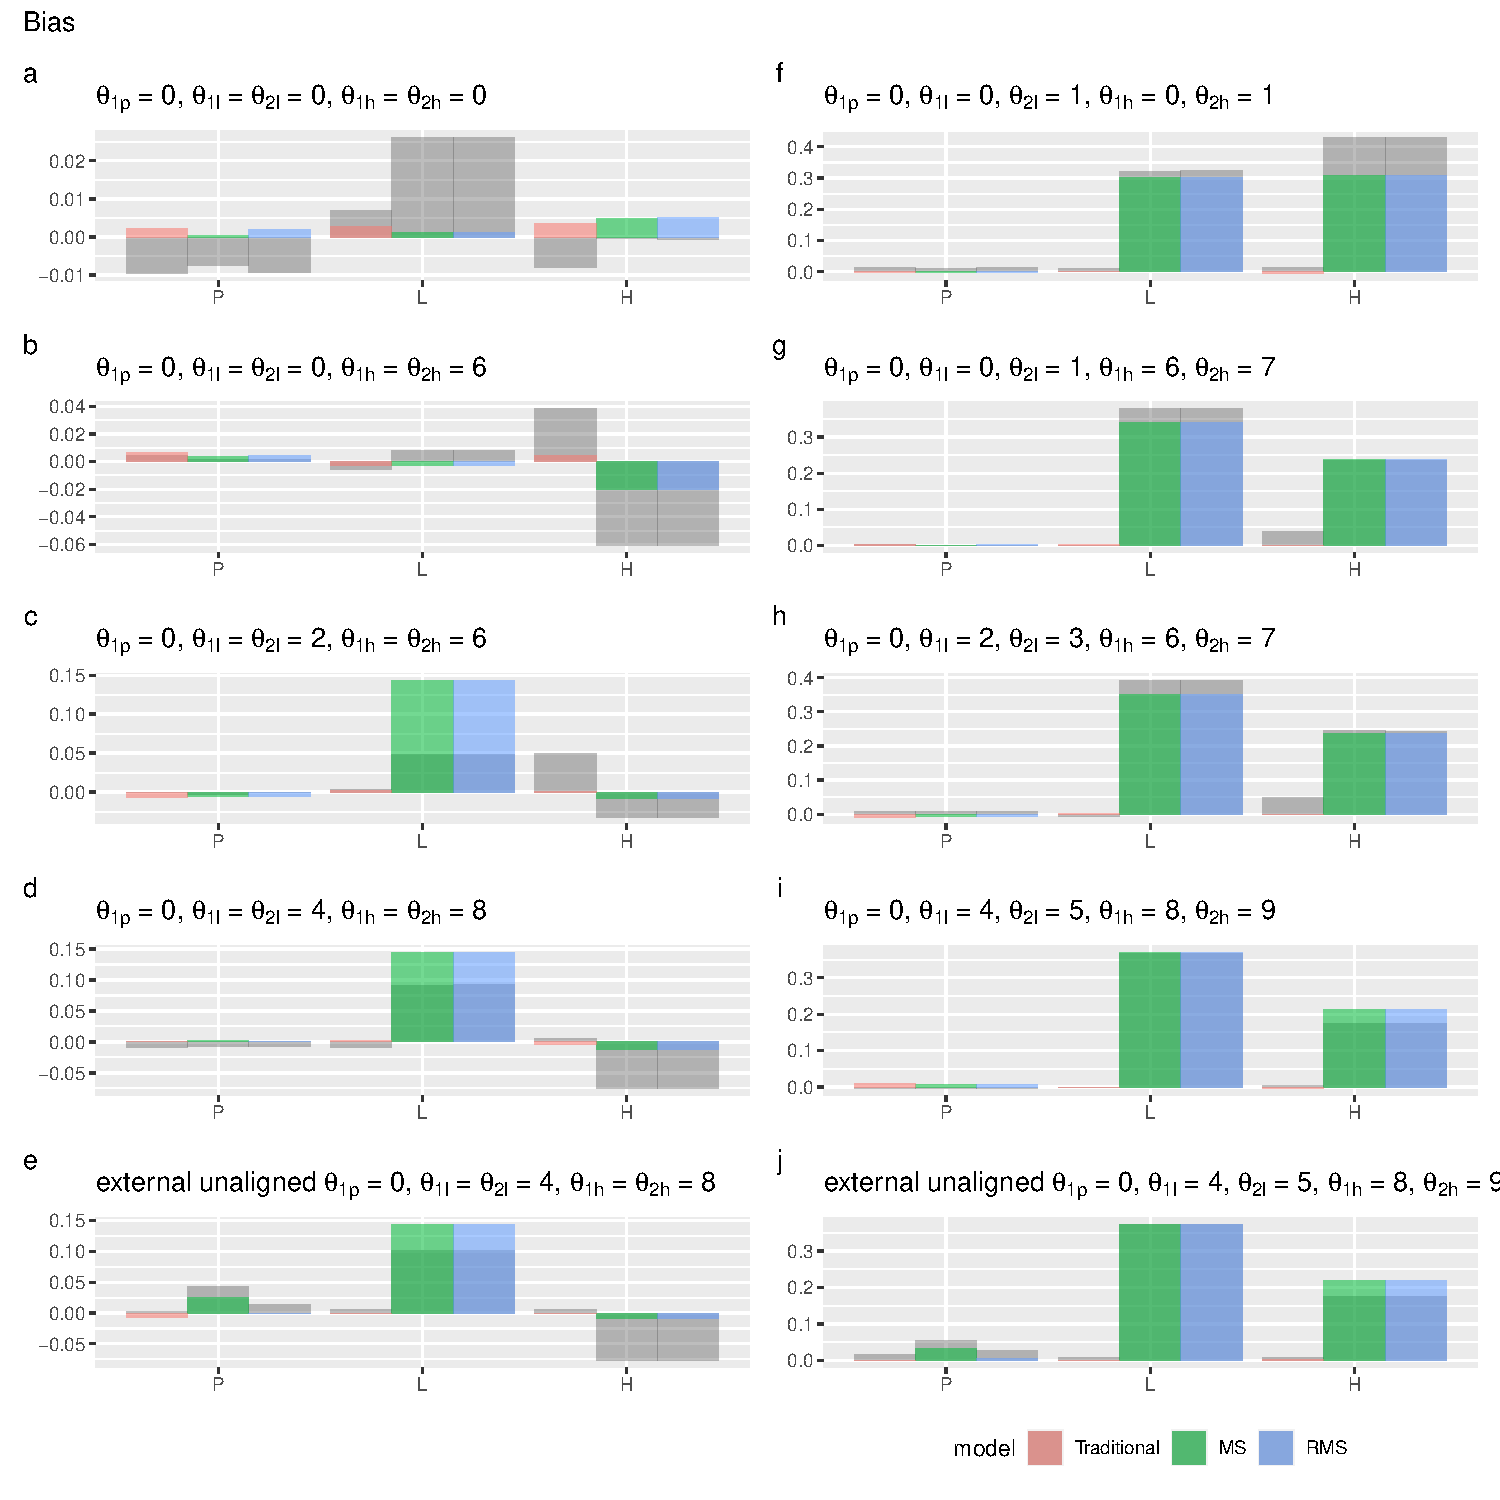
\includegraphics[width=16cm]{chapters/figures/Bias1.pdf}
\caption{Simulated bias for the estimators of $\theta_{1k}$}
\subcaption*{$\theta_{jk}$ is the stage $j$ treatment effect of treatment $k$, where $j = 1,2, k = P, L, H$, P = placebo, L = low dose, and H = high dose. Two hierarchical models: MAC-snSMART (MS) and robust MAC-snSMART (RMS) are compared against the traditional method. The results of total sample size 50 are shown as the colored bars, while the results of total sample size 25 are shown as the overlaying grey bars. The simulation settings are described on the top of each graph, where $\theta_{jk}$ denotes the true value of the expected treatment effects of treatment $k$ in stage $j$, $j = 1, 2$, $k = P, L, H$, and \emph{external unaligned} means the placebo treatment effects in external control data are inconsistent with the placebo treatment effect in the current trial.}
\label{fig:Bias}
\end{figure}

\newpage
\begin{figure}[H]
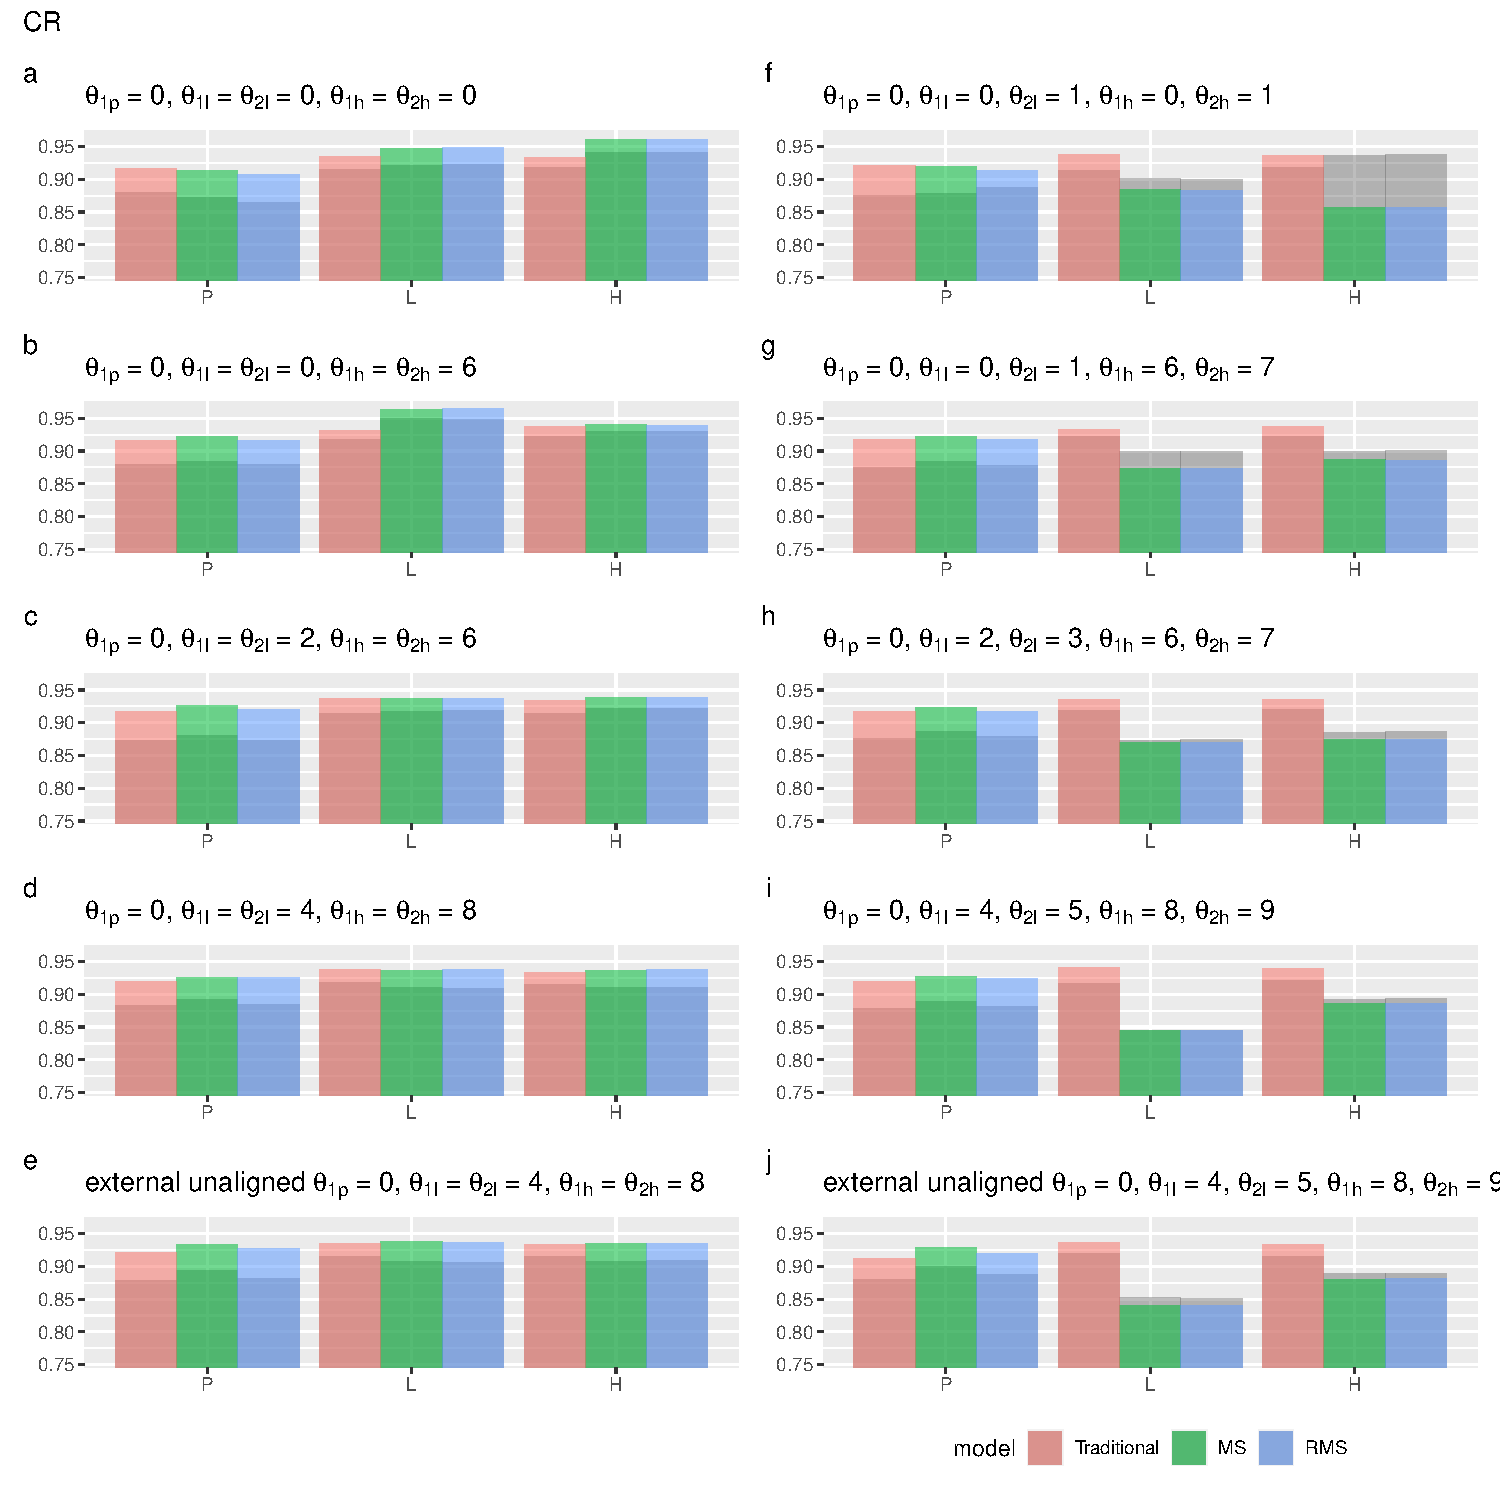
\includegraphics[width=16cm]{chapters/figures/CR.pdf}
\caption{Simulated 95\% coverage rate (CR) for the estimators of $\theta_{1k}$}
\subcaption*{Note: $\theta_{jk}$ is the stage $j$ treatment effect of treatment $k$, where $j = 1,2, k = P, L, H$, P = placebo, L = low dose, and H = high dose. Two hierarchical models: MAC-snSMART (MS) and robust MAC-snSMART (RMS) are compared against the traditional method. The results of total sample size 50 are shown as the colored bars, while the results of total sample size 25 are shown as the overlaying grey bars. The simulation settings are described on the top of each graph, where $\theta_{jk}$ denotes the true value of the expected treatment effects of treatment $k$ in stage $j$, $j = 1, 2$, $k = P, L, H$, and \emph{external unaligned} means the placebo treatment effects in external control data are inconsistent with the placebo treatment effect in the current trial.}
\label{fig:CR}
\end{figure}

\newpage
\begin{figure}[H]
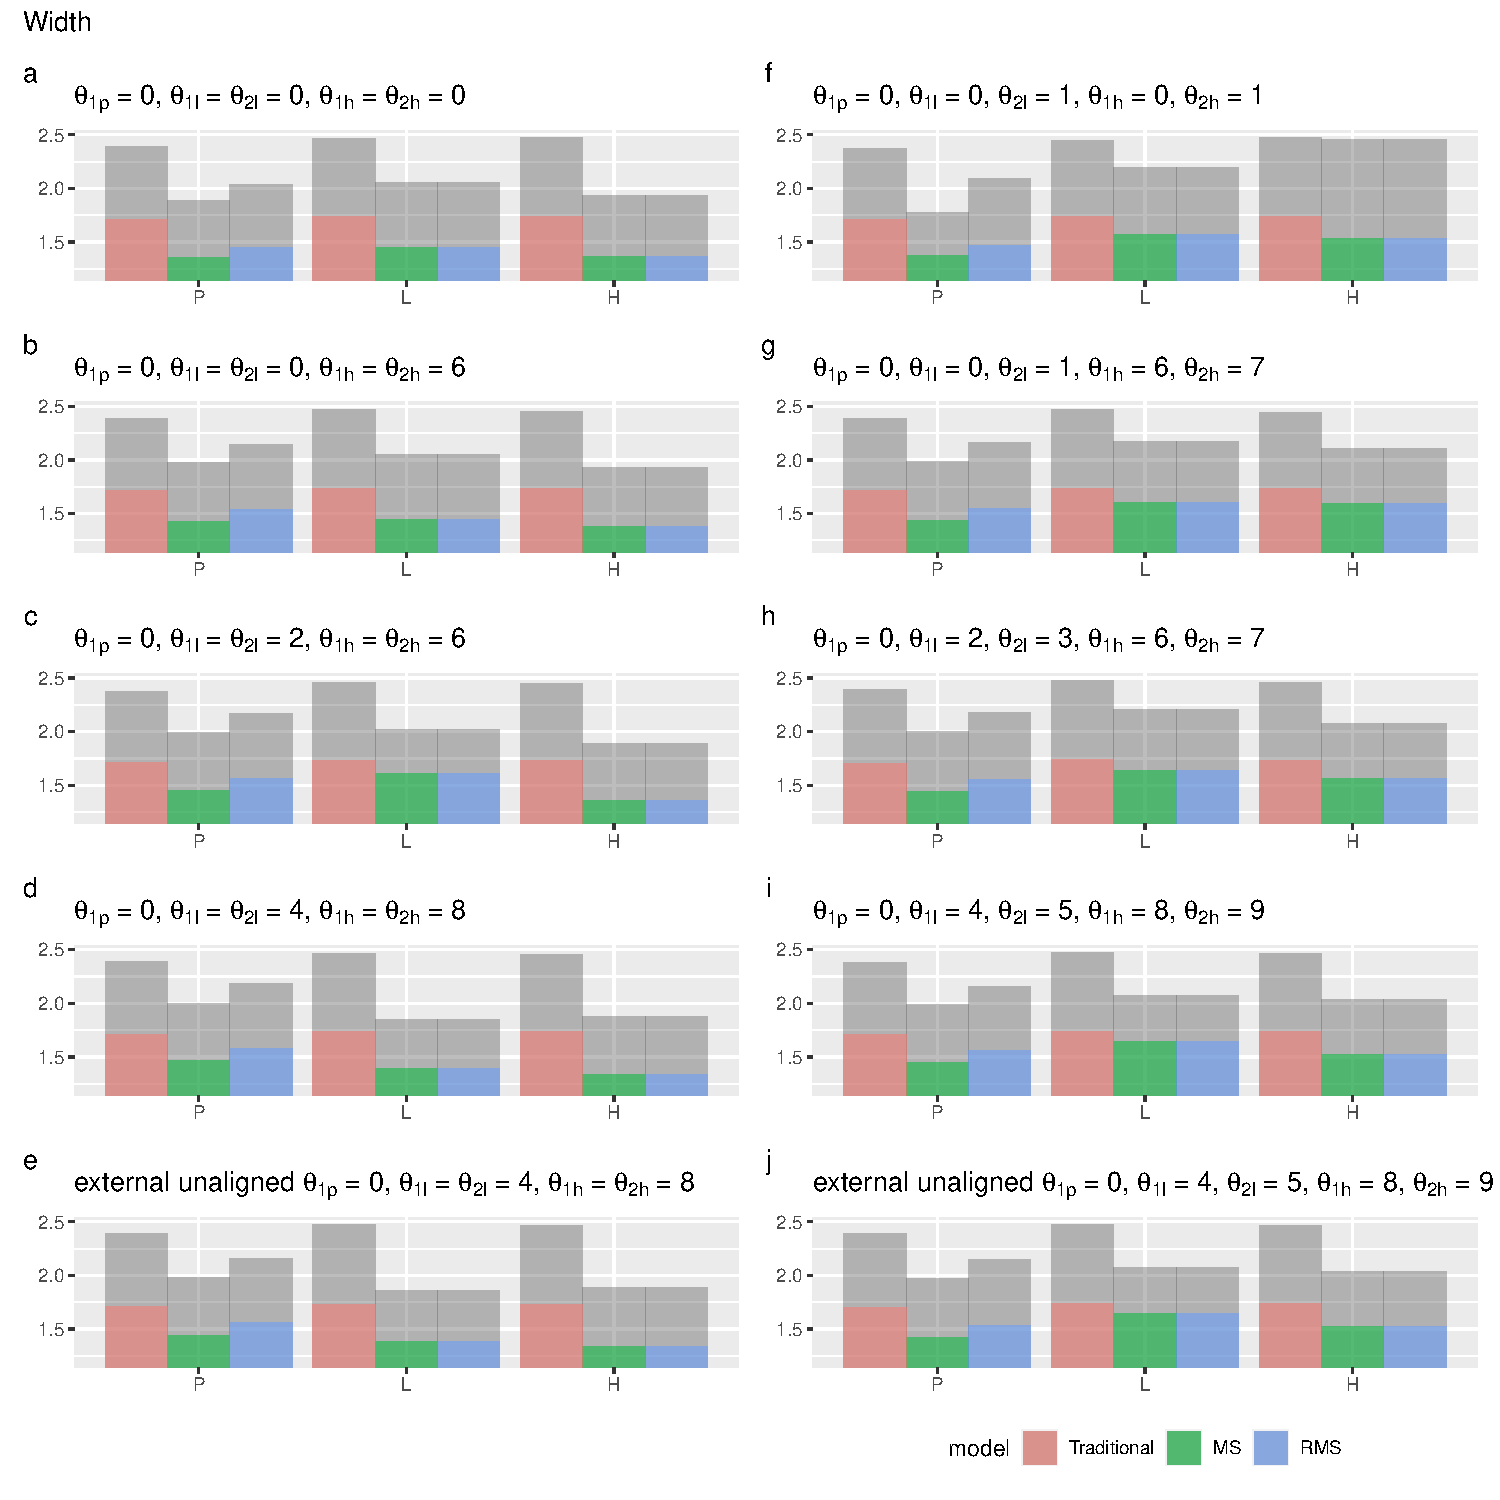
\includegraphics[width=16cm]{chapters/figures/Width.pdf}
\caption{Simulated width for the estimators of $\theta_{1k}$}
\subcaption*{Note: $\theta_{jk}$ is the stage $j$ treatment effect of treatment $k$, where $j = 1,2, k = P, L, H$, P = placebo, L = low dose, and H = high dose. Two hierarchical models: MAC-snSMART (MS) and robust MAC-snSMART (RMS) are compared against the traditional method. The results of total sample size 50 are shown as the colored bars, while the results of total sample size 25 are shown as the overlaying grey bars. The simulation settings are described on the top of each graph, where $\theta_{jk}$ denotes the true value of the expected treatment effects of treatment $k$ in stage $j$, $j = 1, 2$, $k = P, L, H$, and \emph{external unaligned} means the placebo treatment effects in external control data are inconsistent with the placebo treatment effect in the current trial.}
\label{fig:Width}
\end{figure}

Similar trends were observed in simulations with sample sizes of 25. As expected, bias, \ac{rMSE} and \ac{CI} width were larger, and coverage rate was smaller than cases where the total sample size was 50. Notably, \ac{MAC}-snSMART methods still provide negligible bias and more than 90\% coverage rate for low dose and high dose under all scenarios when assumptions are not violated. 

Table \ref{tab:TypeI} and Figure \ref{fig:Power} present the type I error and power of each model. The \ac{MAC}-snSMART methods have smaller type I errors when its assumption of full exchangeability between stages is upheld, and the type I error is still reasonable (below 0.1) when this assumption is violated. The traditional method performs best when the assumptions of \ac{MAC}-snSMART methods are violated. When the treatment effect is $\geqslant 4$, i.e., a clinically meaningful difference in our simulations, all methods have power close to 1 under all scenarios, even when the total sample size is 25. When the treatment effect is equal to 2, the \ac{MAC}-snSMART methods have an increase in power in comparison with the traditional method, especially when the total sample size is small.      

\section{Example Data Analysis} \label{s:example}

To understand the practical utility of the proposed \ac{snSMART} design and \ac{MAC}-snSMART methods, we conducted a reanalysis using the study results of SPITFIRE study. Given that the trial stopped for futility after stage 1, we were only able to obtain summary-level \ac{NSAA} total score and summary-level \ac{6MWD} at baseline and week 48 (details shown in Table \ref{tab:Roche}). To create a dataset that matches our proposed trial design, we simulated stage 1 patient-level data by randomly drawing from normal distributions based on the SPITFIRE data. Here we describe the simulation process for \ac{NSAA} total score in detail. Specifically, 30 patients' outcomes for the placebo arm were represented by drawing from $N(-2.99, 0.65^2 \times \sqrt{30})$, 29 patient outcomes for the low dose arm were represented by drawing from $N(-3.44, 0.67^2 \times \sqrt{29})$, and 33 patient outcomes for the high dose arm were represented by drawing from $N(-2.41, 0.64^2 \times \sqrt{33})$. According to the SPITFIRE study protocol, we set a change of $\geqslant -3.1$ points from baseline as the threshold for a clinically meaningful treatment effect \citep{muntoni2018minimal}. This threshold is also used to categorize stage 1 responders and nonresponders. Stage 2 treatment outcomes were again randomly generated according to formula \ref{eq:joint} with $s_{kk'}$ randomly chosen between -1 and 1, and $Y_{2l} \sim N(-3.44, 0.67^2\sqrt{n_{2l}})$ and $Y_{2h} \sim N(-2.41, 0.64^2\sqrt{n_{2h}})$, for low and high dose, respectively. Our proposed \ac{snSMART} design and randomly generated stage 1 outcomes dictated $n_{2l}$ and $n_{2h}$. We followed the same procedure to simulate stage 1 and stage 2 \ac{6MWD} data.

Given our methods formally incorporate external control data, we used the \ac{CINRG} \ac{DNHS} data as the source of external control in this real-trial motivated example data analysis. Data from participants from the \ac{DNHS} who met the eligibility criteria of the SPITFIRE trial and had \ac{NSAA} total score or \ac{6MWD} records were used for the external control group. Given that the participant visit schedule of \ac{DNHS} was different from the SPITFIRE trial, for each participant, we picked the test record with `days from baseline' closest to 336 ($48 \times 7$) as their `Week 48' record. In the end, for \ac{NSAA} total score, data from 25 participants were included in the external control group with a mean \ac{NSAA} total score change from baseline being -1.04 and its standard deviation being 0.77. Similarly, for \ac{6MWD}, data from 25 participants were included in the external control group with a mean \ac{6MWD} change from baseline being -22.36 and its standard deviation being 27.98.

\begin{table}[H]
\caption{\label{tab:Roche} The SPITFIRE trial Study Measures. Summary
statistics are reported as mean (SD) for NSAA and 6MWD.}
\begin{center}
\begin{tabular}{p{4.8cm}p{3cm}p{2.9cm}p{3cm}}
\centering  & \centering Placebo & \centering RO7239361 Low Dose & \centering RO7239361 High Dose \tabularnewline
\hline
\textit{Baseline} &&&\\
\raggedleft Sample Size & \centering 56 & \centering 55 & \centering 55 \tabularnewline 
\raggedleft NSAA & \centering 23.1  (6.4) & \centering 24.5  (5.5) & \centering 22.7  (6.7) \tabularnewline
\raggedleft 6MWD & \centering 388.33 (69.59) & \centering 399.73 (68.35) & \centering 370.73 (93.35) \tabularnewline
\hline
\textit{Week 48} &&& \tabularnewline
\raggedleft Sample Size - NSAA & \centering 30 & \centering 29 & \centering 33 \tabularnewline 
\raggedleft Changes in NSAA & \centering -2.99  (0.65) & \centering -3.44  (0.67) & \centering -2.41  (0.64) \tabularnewline
\raggedleft Sample Size - 6MWD & \centering 29 & \centering 25 & \centering 31 \tabularnewline 
\raggedleft Changes in 6MWD & \centering -41.3 (8.7) & \centering -39.6 (9.0) & \centering -30.0 (8.7) \tabularnewline
\hline
\end{tabular}
\end{center}
\end{table}

Along with the robust \ac{MAC}-snSMART method, the \ac{BJSM} method \citep{fang2022comparing} was also implemented to analyze the SPITFIRE trial data. The estimators obtained from the \ac{BJSM} are compared with the robust \ac{MAC}-snSMART estimators to see whether our model generates estimates consistent with the \ac{BJSM}.

Given that there is wide variation in outcomes, 30,000 realizations were simulated for both \ac{6MWD} and \ac{NSAA} total score to assess the model performances. We fitted the traditional analytic method, \ac{BJSM}, and robust \ac{MAC}-snSMART method, where the results are shown in Table \ref{tab:comp}. Given that the original result of the SPITFIRE trial was obtained through fitting a \ac{MMRM} and we do not have access to the covariates that were included in that \ac{MMRM} model, it is reasonable for the traditional analytic method to have estimators with slightly larger \ac{CI} width. In fact, if we manually calculate the \ac{6MWD} \ac{CI} width based on the data in Table \ref{tab:Roche} through $1.7 \pm 1.96 \times \sqrt{8.7^2 + 9.0^2}$ and $11.3 \pm 1.96 \times \sqrt{8.7^2 + 8.7^2}$, we would obtain $(-22.83, 26.23)$ and $(-12.82, 35.42)$, which are almost the same with the \ac{6MWD} \ac{CI} obtained from the traditional analytic method. The same applies to \ac{NSAA} total score. Notice that the estimators obtained from the robust \ac{MAC}-snSMART method and \ac{BJSM} are consistent with each other and have significantly smaller \ac{CI} width than the traditional method because of the efficient use of data across both stages. 

\begin{table} 
\caption{\label{tab:comp} Example Data Analysis Result Comparison}
\begin{center}
%\begin{tabular}{p{2.6cm}p{3.3cm}p{3.3cm}p{3.3cm}p{3.3cm}}
\begin{tabular}{ccccc}
Estimator &  Original Result &  Traditional &   BJSM &  RMS  \tabularnewline
\hline
\multicolumn{1}{l}{\textit{NSAA}} &&&&\\
\multicolumn{1}{r}{$\hat{\theta}_{1p}$} &  -2.99 (-4.26, -1.71) &  -2.98 (-4.24, -1.73) &  -2.91 (-4.01, -1.82) &  -2.89 (-3.68, -2.10) \tabularnewline 

\multicolumn{1}{r}{$\hat{\theta}_{1l}$}  &  -3.44 (-4.75, -2.13) &  -3.44 (-4.74, -2.14) &  -3.38 (-4.34, -2.41) &  -3.40 (-4.49, -2.31)  \tabularnewline

\multicolumn{1}{r}{$\hat{\theta}_{1h}$} &  -2.41 (-3.66, -1.16) &  -2.41 (-3.65, -1.17) &   -2.42 (-3.35, -1.48) &  -2.49 (-3.56, -1.42) \tabularnewline

\multicolumn{1}{r}{$\hat{\theta}_{1l} - \hat{\theta}_{1p}$} &  -0.45 (-2.17, 1.27) &  -0.46 (-2.27, 1.36) &  -0.46 (-1.91, 0.98) &  -0.52 (-1.88, 0.83)   \tabularnewline
\multicolumn{1}{r}{$\hat{\theta}_{1h} - \hat{\theta}_{1p}$} &  	0.58 (-1.10, 2.26) &  0.58 (-1.20, 2.35) &  0.50 (-0.93, 1.92) &  0.40 (-0.94, 1.74) \tabularnewline
\hline
\multicolumn{1}{l}{\textit{6MWD}} &&&&\\
\multicolumn{1}{r}{$\hat{\theta}_{1p}$} &  -41.3 (-58.4, -24.2) &  -41.3 (-58.2, -24.5) &  -41.1 (-54.4, -27.8) &  -41.0 (-52.5, -29.3) \tabularnewline 

\multicolumn{1}{r}{$\hat{\theta}_{1l}$} &  -39.6 (-57.2, -22.0) &  -39.6 (-57.0, -22.2) &  -39.3 (-51.6, -27.6) &  -39.4 (-53.2, -26.1)  \tabularnewline

\multicolumn{1}{r}{$\hat{\theta}_{1h}$} &  -30.0 (-47.1, -12.9) &  -30.0 (-46.7, -13.0) &   -29.7 (-40.8, -18.7) &  -30.2 (-42.1, -18.0) \tabularnewline

\multicolumn{1}{r}{$\hat{\theta}_{1l} - \hat{\theta}_{1p}$} &  1.7 (-21.1, 24.6) &  1.8 (-22.6, 26.0) &  1.8 (-16.6, 19.5) &  1.6 (-15.6, 19.1)    \tabularnewline
\multicolumn{1}{r}{$\hat{\theta}_{1h} - \hat{\theta}_{1p}$} &  11.3 (-11.0, 33.6) &  11.5 (-12.5, 35.4) &  11.4 (-5.8, 28.6) &  10.9 (-6.4, 28.1) \tabularnewline
\hline
\end{tabular}
\end{center}
\begin{tablenotes}
      \small
      \item Note: $\hat{\theta}_{1k}$ is the estimated stage 1 treatment effect for treatment $k$, $k = P,L,H$. Four analytic methods: original SPITFIRE trial results, traditional analytic method, Bayesian joint stage modeling (BJSM), and robust MAC-snSMART (RMS) are compaired. The confidence or credible intervals of the estimates are shown in the parenthesis.
\end{tablenotes}
\end{table}

\section{Discussion} \label{s:discuss}
In this paper, we were motivated by the rare disease setting of \ac{DMD} and the SPITFIRE trial to present an alternative design and methods with more efficient use of second stage data. We have proposed a robust \ac{MAC}-snSMART method to estimate the treatment effect of placebo, low and high doses from an \ac{snSMART} design with a continuous outcome of interest. Our proposed \ac{snSMART} design and robust \ac{MAC}-snSMART method are highly responsive to the \ac{FDA}'s Complex Innovative Design program \citep{fdaCID}. We have provided guidelines for prior distributions, sensitivity analyses to assumptions of the models, and comparator models which an investigator or sponsor can provide to regulatory officials to illustrate the efficiency and robustness of the robust \ac{MAC}-snSMART method for an \ac{snSMART} design. The robust \ac{MAC}-snSMART method provides the most accurate and robust estimators when the expected treatment effect of the same dose level follows the same normal distribution across stages. 

Our \ac{snSMART} design and this assumption of the robust \ac{MAC}-snSMART method that treatment effects of the same dose level follow the same normal distribution across arms is most appropriate for diseases that stay relatively stable throughout the trial period, and when there is no treatment effect, patients' primary outcomes do not fluctuate dramatically. Diseases like \ac{DMD} used as motivation here, corticobasal degeneration (CBD), and familial Mediterranean fever (FMF), which are slower to progress, are good candidates for our \ac{snSMART} design and methods. The proposed robust \ac{MAC}-snSMART method assumes treatment effects from the first and second stages are exchangeable which incorporates this assumption of a stable disease and assumes a stable treatment effect with an adequate washout period between stages 1 and 2. If first and second stage treatment effects are not similar across stages or there is not an adequate washout period, a multi-stage design and robust exchangeable model may not be appropriate and lead to biased estimation of treatment effects as we saw in the deteriorating performance of the robust \ac{MAC}-snSMART method results under the second data generation process. At the end of the trial, sensitivity analyses comparing results from the traditional analytic method can be compared to the robust \ac{MAC}-snSMART method to assess these assumptions. 

It is possible that even a high dose of the treatment being investigated cannot provide a clinically meaningful treatment effect by the end of stage 1. Under this scenario, it will not be ethical to continue the trial for those who received high dose in stage 1. Hence, we recommend that if less than 30\% of patients responded to high dose in stage 1, stage 2 will not be conducted, and all treatment effects will be calculated based on stage 1 outcome only.

The \ac{MAC}-snSMART method provides significant power gains compared to two-sample t-tests, which are commonly used in \ac{DMD} trials. For example, under simulation scenario 2 ($\theta_p < \theta_l = 2 < \theta_h = 6$), with $s_{1p} = 1.5, s_{1l} = 2, n_{1p} = 10, n_{1l} = 20$ and $\alpha=0.05$, a one-sided two-sample t-test can only achieve a power of 0.89, while our simulation shows that \ac{MAC}-snSMART methods can achieve a power higher than 0.95 (Figure \ref{fig:Power}). The power gain is even more significant in smaller samples. When $n_{1p} = 5, n_{1l} = 10$, the power of a t-test can only reach 0.62 while the power of \ac{MAC}-snSMART method can reach 0.76 (Figure \ref{fig:Power}). This demonstrates that our proposed trial design and method are useful for obtaining a higher level of evidence for efficacy in rare disease dose-finding trials.

All of our simulations adopted the 1:2:2 placebo, low dose, and high dose randomization ratio in stage 1. A randomization ratio of 1:3:3 can be used when external control data is (almost) fully exchangeable with the current trial placebo data. With a smaller proportion of participants being randomized to the placebo arm in stage 1, the external control data will have a stronger impact than the current trial placebo data on the estimation of the placebo treatment effect. 

In our simulations, we generated five sets of summary-level external control data in each realization, which may or may not be consistent with the available placebo data in a current trial. Due to between-trial heterogeneity, the amount of effective external control data information is not simply the number of external control data placebo subjects, it must be a smaller number. We see in our example data analysis that the robustified summary-level natural history data of 25 participants is roughly equivalent to an effective sample size of 12. In general, if one set of external control data and current trial data are in clear conflict, this set of external control data will not help improve the placebo effect estimation. Thus more data contributing to the placebo will not always be useful for decreasing the number of patients needed on the placebo arm. 

\begin{figure}[H]
\centerline{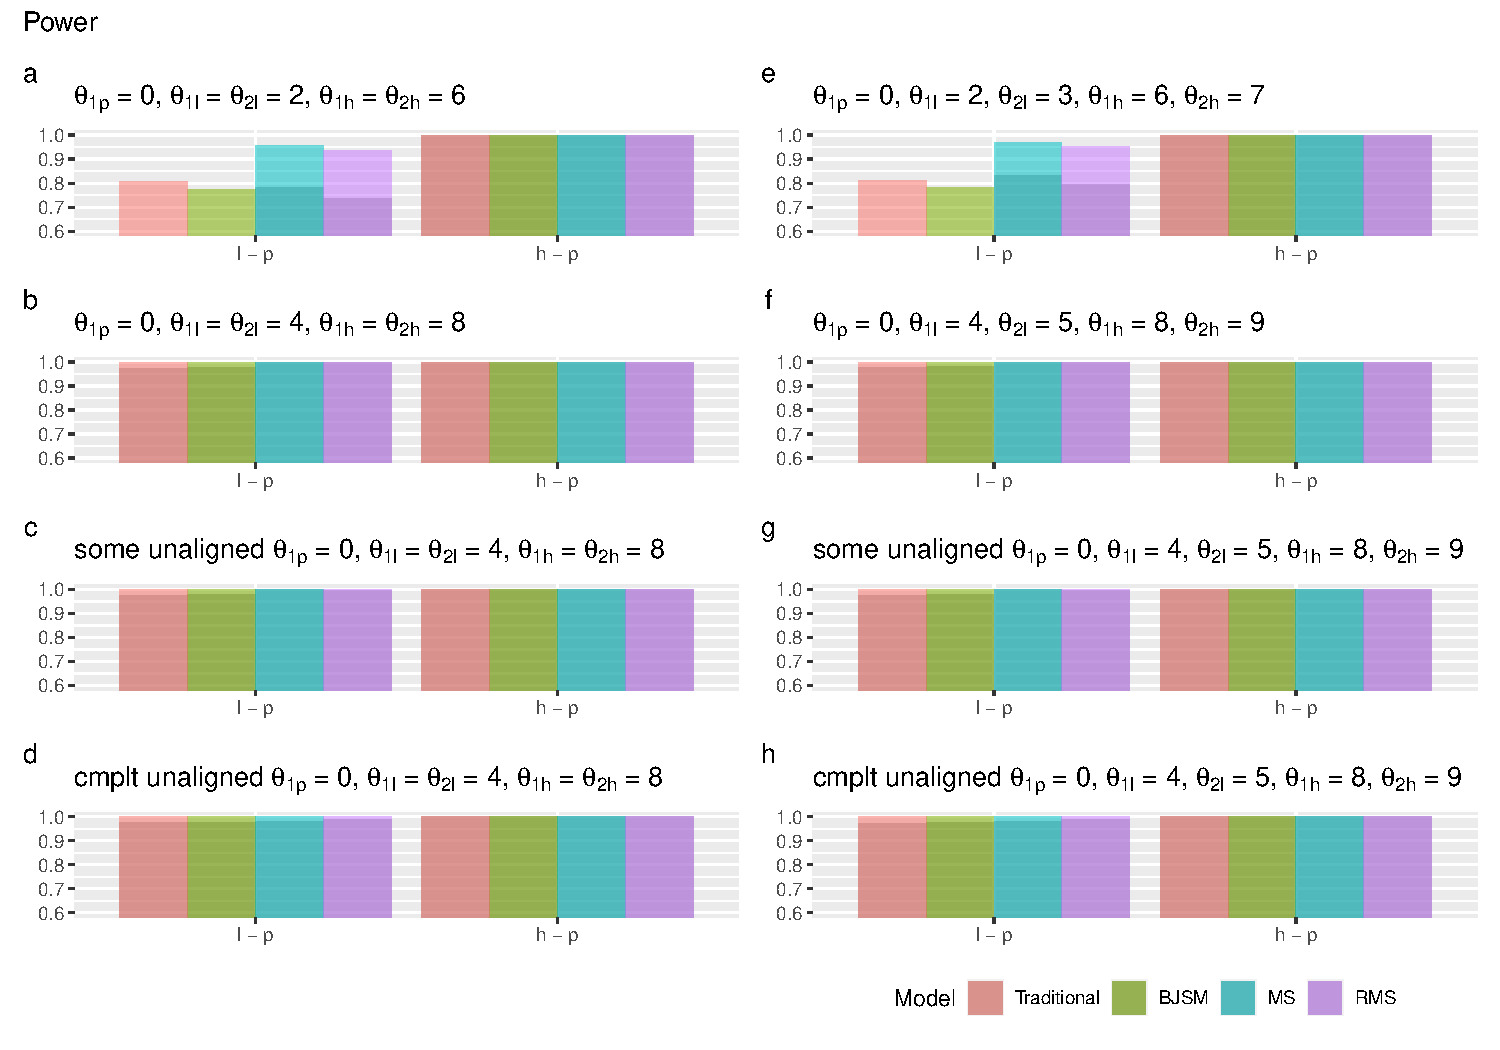
\includegraphics[width=16cm]{chapters/figures/CRpower.pdf}}
\caption{Simulated power of the MAC-snSMART methods}
\subcaption*{In this paper, the power is defined as the probability that the credible intervals of $\hat{\theta}_{1l} - \hat{\theta}_{1p}$ and $\hat{\theta}_{1h} - \hat{\theta}_{1p}$ do not include 0 when there are treatment effect difference between low dose and placebo and high dose and placebo. Two hierarchical models: MAC-snSMART (MS) and robust MAC-snSMART (RMS) are compared against the traditional method. The results of total sample size 50 are shown as the colored bars, while the results of total sample size 25 are shown as the overlaying grey bars. The simulation settings are described on the top of each graph. $\theta_{jk}$ denotes the true value of the expected treatment effects of treatment $k$ in stage $j$, where $j = 1, 2$, $k = P, L, H$, P = placebo, L = low dose, and H = high dose. \emph{external unaligned} means the placebo treatment effects in external control data are inconsistent with the placebo treatment effect in the current trial.}
\label{fig:Power}
\end{figure}

Our proposed robust MAC-snSMART method assumes fully exchangeable treatment effects across trial stages, and allows for differential heterogeneity and nonexchangeability in external control data. This method can be easily extended to include treatment effect nonexchangeability for low dose and high dose across trial stages.

The SPITFIRE trial and many other \ac{DMD} trials incorporate participant demographic and baseline characteristics covariates in their analysis. In the future, we hope to extend the \ac{snSMART} design and robust \ac{MAC}-snSMART method to include patient-level covariates and add an interim analysis at the end of stage 1, e.g., stopping for futility or dropping a treatment arm. In addition, data in \ac{DMD} trials is usually collected in a longitudinal manner with 3 or more visits. Future work can incorporate longitudinal data into our design and methods. 